%%%%%%%%%%%%%%%%%% USAGE INSTRUCTIONS %%%%%%%%%%%%%%%%%%
% - Compile using LuaLaTeX and biber, unless there is a particular reason not to. Do not use the older LaTex/PDFLaTeX or BibTeX. (The fonts won't work correctly.)
% - Expect to get 2 warnings when working correctly, one on xcolor and hyperref, and one on ExtSizes saying is better to use a class. These can be ignored.
% - Font and the report 'year' must be specified when all \documentclass or the template won't work correctly. (There's no error checking/default cases!)
% - For best performance save images/graphics as PDF files, not as png/jpg/eps. This makes no difference to how images are inserted using \includegraphics.
% - As many further packages as wanted can be loaded. Below are just an example set. Note that template itself loads a number of packages, including hyperref.
% - References are handed using biblatex.
% - Link to the presentation of dissertations policy: https://documents.manchester.ac.uk/display.aspx?DocID=2863



%%%%%%%%%%%%%%%%%% META DATA SETUP %%%%%%%%%%%%%%%%%%
% This is where the document title and author are set. Other details for the title page are set later
% Note that if/when you edit these you may need to 'Recompile from scratch' to get the changes to display in the PDF. (In Overleaf, select the down arrow to the right of the 'Recompile' button)
\begin{filecontents*}{\jobname.xmpdata}
  \Title{Football Computer Vision AI} 
  \Author{Maanav Chauhan \\ 11109655} % should be student number rather than name to help with annoymous marking
  \Language{en-GB}
  \Copyrighted{True}
  % More meta-data fielda can be added here if wanted, see https://ctan.org/pkg/pdfx?lang=en for fields
\end{filecontents*}


%%%%%%%%%%%%%%%%%% DOCUMENT SETUP %%%%%%%%%%%%%%%%%%
\documentclass[11pt,bsc]{uom_eee_dissertation_casson} 
% course can be bsc or beng
% Check your course handbook for the correct font size to use. Make sure this is correct - you may get an overlength penalty if not! Is currently 12 for BEng, and 11 for bsc. The template doesn't change this automatically for you



%%%%%%%%%%%%%%%%%% PACKAGES AND COMMANDS %%%%%%%%%%%%%%%%%%

% Packages
\usepackage{csquotes} % For better quotation formatting
\usepackage{graphicx}              % for adding graphics files
  \graphicspath{ {./images/} }
\usepackage{amsmath}               % assumes amsmath package installed
  \allowdisplaybreaks[1]           % allow eqnarrays to break across pages
\usepackage{amssymb}               % assumes amsmath package installed 
\usepackage{url}                   % format hyperlinks correctly
\usepackage{rotating}              % allow portrait figures and tables
\usepackage{multirow}              % allows merging of rows in tables
\usepackage{lscape}                % allows pages to be typeset in landscape mode
\usepackage{tabularx}              % allows fixed width tables
\usepackage{verbatim}              % enhanced version of built-in verbatim environment
\usepackage{footnote}              % allows more control over footnote environments
\usepackage{float}                 % allows H option on floats to force here placement
\usepackage{booktabs}              % improve table line spacing
\usepackage{lipsum}                % for adding dummy text here
\usepackage[base]{babel}           % required for lisum package
\usepackage{subcaption}            % for multiple sub-figures in a single float
\usepackage{siunitx}               % add SI units
% Add your packages here
% \documentclass{article}
\usepackage{amsmath}
\usepackage{url}
\usepackage{algorithm2e}
\usepackage{cite}
\usepackage{enumitem}
\usepackage{booktabs} % Include in the preamble


% Custom commands
\newcommand{\degree}{\ensuremath{^\circ}}
\newcommand{\sus}[1]{$^{\mbox{\scriptsize #1}}$} % superscript in text (e.g. 1st)
\newcommand{\sub}[1]{$_{\mbox{\scriptsize #1}}$} % subscript in text
\newcommand{\otoprule}{\midrule[\heavyrulewidth]}
\newcolumntype{Z}{>{\centering\arraybackslash}X}  % tabularx centered columns 
% Add your custom commands here



%%%%%%%%%%%%%%%%%% REFERENCES SETUP %%%%%%%%%%%%%%%%%%

% Setup your references here. Change the reference style here if wanted
\usepackage[style=ieee,backend=biber,backref=true,hyperref=auto,maxbibnames=3,minbibnames=1,sorting=none,style=numeric]{biblatex}

% Note backref=true adds a page number (and hyperlink) to each reference so you can easily go back from the references to the main document. You may prefer backref=false if you need to stick strictly to a given reference style


% Fixes which can't be applied in the .cls file
\DefineBibliographyStrings{english}{backrefpage = {cited on p\adddot},  backrefpages = {cited on pp\adddot}}
%  \renewcommand*{\bibfont}{\large}


% Add more .bib files here if wanted
\addbibresource{references.bib}



%%%%%%%%%%%%%%%%%% AUTOMATIC WORD COUNT SETUP %%%%%%%%%%%%%%%%%%
% Automatically counts the words present and makes a \mywordcount variable. This is used later to automatically add the word count (which can be overridden if wanted)
% See https://www.overleaf.com/learn/how-to/Is_there_a_way_to_run_a_word_count_that_doesn%27t_include_LaTeX_commands%3F for info on what words are counted and how to control this. Any changes to what's counted need to be made in uom_thesis_casson.cls, in the \newcommand{\quickwordcount} command. The default doesn't count words in headings, captions, or references and so you may get slightly different numbers if use a different word count tool
% This can be a bit fragile. If it doesn't work, there's an option later on to just type in a numer
\quickwordcount{\currfilebase} % run word count. This just counts the words. Is displayed with the \wordcount command later



%%%%%%%%%%%%%%%%%% START DOCUMENT %%%%%%%%%%%%%%%%%%

% Don't edit these lines, title and author are automatically taken from the document meta-data defined above

\begin{document}
\makeatletter
\title{\xmp@Title}
\studentid{\xmp@Author}
\makeatother

% Set the below yourself
\course{Computer Science}

\faculty{Science and Engineering} % "Faculty of" is added automatically
\school{School of Engineering} 
\submitdate{2025} % regulations ask only for the year, not month
% \wordcount{\mywordcount}
\wordcount{13819}
\maketitle



%%%%%%%%%%%%%%%%%% LISTS OF CONTENT %%%%%%%%%%%%%%%%%%
\uomtoc
\uomlof
\uomlot
\newpage
\section*{List of Abbreviations}
\begin{description}[align=left, labelwidth=3cm]
  % \item[API] Application Programming Interface
  \item[AssA] Association Accuracy
  \item[BGR] Blue-Green-Red (colour space)
  \item[CNN] Convolutional Neural Network
  \item[DetA] Detection Accuracy
  \item[DLT] Direct Linear Transformation
  \item[DPM] Deformable Part Model
  \item[FPS] Frames Per Second
  \item[HSV] Hue, Saturation, Value (colour space)
  \item[HOTA] Higher Order Tracking Accuracy
  \item[ID] Identifier
  \item[IoU] Intersection over Union
  \item[KMeans] K-Means Clustering
  \item[MOTA] Multiple Object Tracking Accuracy
  \item[NMS] Non-Maximum Suppression
  \item[OCR] Optical Character Recognition
  \item[RGB] Red, Green, Blue (colour space)
  \item[ROI] Region of Interest
  \item[SORT] Simple Online Real-time Tracking
  \item[SVD] Singular Value Decomposition
  \item[SVM] Support Vector Machine
  \item[UMAP] Uniform Manifold Approximation and Projection
  \item[YOLO] You Only Look Once
\end{description}


%%%%%%%%%%%%%%%%%% ABSTRACT %%%%%%%%%%%%%%%%%%
\begin{abstract} 

With the constant growing demand and love for the game of football, the interest for tactical analysis, performance evaluation, and enhanced viewer experiences has also increased significantly. This project develops a system for the automated detection and tracking of football players, referees, and the football during the game. It achieves this by building upon state-of-the-art object detection models and tracking algorithms.

For real-time object detection, the system leverages YOLO (You Only Look Once). On the other hand, K-Means Clustering and the SIGLIP Model are used for player team classification, whereas, ByteTrack is used to obtain an overall robust multi-object tracking system. 

The system further goes on to generate a Bird's Eye View using the concepts of homography. This plays a key role in generating heatmaps and off-side lines which can be of great aid for spatial and tactical analysis. The system also does a comprehensive analysis, returning the speed and distance travelled by each player during the match.

This work highlights the potential of deep learning-based methods in advancing sports analytics and lays the core foundation upon which, further enhancements such event recognition, action recognition, and integration with match analysis can be built.
\end{abstract}
\clearpage



%%%%%%%%%%%%%%%%%% DECLARATIONS %%%%%%%%%%%%%%%%%%
\begin{uomoriginality}
  \uomoriginalitydeclaration 
  % If the standard originality decalaration is sufficient, saying no portion of the work has been submitted in support of an application for another degree or qualification, the above command will automatically add the required text and nothing else is needed in this section.
  % If the standard statment isn't sufficient, then comment out the \uomoriginalitydeclaration command and type in your own text here explaining the authorship of any re-used portions.
  \section*{Declaration of AI}
  AI was only used for language refinement in a limited amount.
\end{uomoriginality}

\uomcopyrightstatement



%%%%%%%%%%%%%%%%%% ACKNOWLEDGEMENTS %%%%%%%%%%%%%%%%%%
\begin{uomacknowledgements}
I would like to express my sincerest gratitude to everyone who has supported me throughout the course of this project. I am especially thankful to my supervisor, Prof. Afroditi Galata, for her valuable guidance, feedback, and encouragement at every stage of the project. Her insights were instrumental in shaping the direction of this project and overcoming technical challenges.

I would also like to thank the Department of Computer Science for providing the necessary resources and academic environment that made this project possible. Special thanks to my peers and friends for their helpful discussions and moral support, and to the creators of Roboflow and the developers of YOLO and ByteTrack, whose tools and open-source contributions formed the backbone of this implementation.

Finally, I am grateful to my family for their constant encouragement and patience throughout this journey.
\end{uomacknowledgements}



%%%%%%%%%%%%%%%%%% Start content %%%%%%%%%%%%%%%%%%
\uomstartmainbody % Don't delete. used to flag to the hyperlinks in the PDF that the main content is  starting



%%%%%%%%%%%%%%%%%% INTRODUCTION %%%%%%%%%%%%%%%%%%
\section{Introduction} \label{sec:intro}
\subsection{Motivation}




The game of \textit{football} is one of the most globally celebrated and commercially significant sports, capturing the attention of millions of fans and analysts worldwide. With the growth of advanced analytics seen in the recent years, there has been a marked shift in how teams, broadcasters, and fans engage with the game. Football Clubs have started to rely deeply on data-driven insights for overall performance evaluation, tactical analysis, and even individual player development. Similarly, broadcasters and sports technology firms are seeking more automated and intelligent ways of delivering richer, real-time insights to their audiences. At the core of many of these efforts lies the ability to accurately detect, track, and analyse the movements of players and the ball throughout a match.

The motivation for this project stems from the challenge and opportunity of applying computer vision and deep learning techniques to this fast-paced, dynamic environment. Football poses multiple unique problems for visual tracking: players often do occlude one another, lighting and camera angles can vary severely, and the ball itself is small and moves unpredictably and at a fast pace. Despite these challenges, solving this problem has the potential to unlock high-impact use cases; from automatic event detection and tactical heatmaps to advanced player metrics and broadcast enhancements.

This project seeks to develop a robust system that leverages object detection and tracking algorithms (such as \textit{YOLO} and \textit{ByteTrack}) to identify and follow players and the ball in football footage. By focusing on football, the project not only contributes to the technical field of computer vision but also addresses a real-world need in sports technology. The use of machine learning in football analytics is still an evolving area, and there is a clear demand for systems that can operate efficiently, accurately, and with minimal human intervention.

In pursuing this project, the goal is not only to implement existing methods but also to understand their limitations, explore ways to improve tracking reliability, and make contributions that could eventually scale to professional use. Ultimately, this work is driven by both, a technical curiosity about complex visual systems and a deep passion for football, a sport where every movement counts.


\newpage

\subsection{Aims \& Objectives}
This project aims to develop a state-of-the-art system with great accuracy and efficiency, producing comprehensive video analysis. The objectives are summarized as follows:
\begin{enumerate}
    \item Implementing an advanced object detection model to accurately identify the players, referees, the ball, and the pitch.
    \item Utilizing a robust tracking algorithm to maintain consistent player identities across the video frames, despite occlusion or the player leaving and re-entering the pitch.
    \item Differentiating between the two opposing teams using clustering techniques.
    \item Mapping player positions from video frames onto an animated pitch for strategic analysis.
    \item Showcasing the player with possession of the football and the number of successful passes a team completes during the match.
    \item Generating heatmaps to visualize player movements and game dynamics.
    \item Detecting if any team commits and off-side during the match video.
    \item Evaluating the system’s performance across various metrics, including detection accuracy and tracking consistency.
\end{enumerate}

\subsection{Report Structure}
This report outlines the development of a comprehensive football video analytics system that integrates player detection, tracking, team classification, spatial analysis, and tactical analysis. The report is structured as follows:

\begin{enumerate}
    \item \textbf{Chapter 1: Introduction} \\
    The introduction chapter introduces the project and the motivation behind this project. It outlines the aims and key objectives as well, and provides a brief description of the structure of the report.

    \item \textbf{Chapter 2: Background} \\
    This chapter reviews prior work in the areas of sports analytics, object detection, multi-object tracking, team classification, pitch homography, and spatial analysis. It further delves into the theoretical foundations of concepts and algorithms used in the project.

    \item \textbf{Chapter 3: Design}
    \begin{itemize}
        \item \textbf{3.1 System Architecture Overview} \\
        High-level pipeline: object detection $\rightarrow$ tracking $\rightarrow$ classification $\rightarrow$ homography $\rightarrow$ analytics.
        
        \item \textbf{3.2 Data Collection and Annotation} \\
        Describes the dataset, annotation tools (e.g., Roboflow), and labelling schema.

        \item \textbf{3.3 Object Detection} \\
        Details the YOLO model fine-tuning process and its usage for player, referee, ball, and pitch detection.

        \item \textbf{3.4 Multi-Object Tracking} \\
        Explains the choice of ByteTrack for identity tracking and how it integrates with detection.

        \item \textbf{3.5 Team Classification} \\
        Discusses the use of deep embeddings (e.g., SigLIP), clustering (UMAP + K-Means), and team assignment.

        \item \textbf{3.6 Pitch Homography} \\
        Describes the projection of the frame coordinates to a top-down view using homography.

        \item \textbf{3.7 Spatial and Tactical Analysis} \\
        Includes analysis modules like ball possession estimation, offside detection, Voronoi diagram generation, player speed and distance tracking, and pass detection.
    \end{itemize}

    % \item \textbf{Chapter 4: Implementation} \\
    % Covers the software tools and platforms (e.g., PyTorch, OpenCV, Roboflow), modular code design, and any user interface or visualization frameworks used.

    \item \textbf{Chapter 4: Evaluation and Results} \\
    Presents both qualitative and quantitative evaluation of the overall system: mAP scores, tracking metrics, clustering accuracy, and visual results.

    % \item \textbf{Chapter 6: Discussion} \\
    % Reflects on the system's performance, discusses key achievements, limitations, and implications for real-world deployment.

    \item \textbf{Chapter 5: Conclusion} \\
    Summarizes the key outcomes, reiterates the contributions, and comments on the impact of the work. Explores potential improvements such as integrating transformer-based models, enhancing re-identification, and real-time system deployment.

    \item \textbf{References} \\
    All cited works are listed.

    % \item \textbf{Appendices} \\
    % Includes supplementary materials such as full code listings, additional figures, evaluation logs, annotation examples, and system instructions.
\end{enumerate}



%%%%%%%%%%%%%%%%%% BACKGROUND %%%%%%%%%%%%%%%%%%
\newpage
\section{Background} \label{sec:background}



This chapter present a detailed evaluation of each component of the system; player detection, pitch detection, team classification, and tracking performance. Several hyper-parameters have been experimented with to obtain the optimum fine-tuned model for each component. Metrics such as \textbf{mean Average Precision (mAP)} and \textbf{Higher Order Tracking Accuracy (HOTA)} have been used to quantify performance.

\subsection{Common Metrics}
For the evaluation of different components, several different metrics were used. Some of the common ones are explained here briefly:
\begin{enumerate}
    \item \textbf{Accuracy} measures the proportion of correctly predicted instances (both true positives and true negatives) among all instances.
\begin{equation}
\text{Accuracy} = \frac{TP + TN}{TP + TN + FP + FN}
\end{equation}

\item \textbf{Precision} measures the proportion of true positive predictions among all positive predictions.
\begin{equation}
\text{Precision} = \frac{TP}{TP + FP}
\end{equation}

\item \textbf{Recall} (also known as Sensitivity or True Positive Rate) measures the proportion of true positives among all actual positives.
\begin{equation}
\text{Recall} = \frac{TP}{TP + FN}
\end{equation}

\item \textbf{F1 Score} is the harmonic mean of Precision and Recall, providing a balance between the two.
\begin{equation}
\text{F1 Score} = 2 \times \frac{\text{Precision} \times \text{Recall}}{\text{Precision} + \text{Recall}}
\end{equation}

\noindent
Where:
\begin{itemize}
    \item \( TP \) = True Positives
    \item \( TN \) = True Negatives
    \item \( FP \) = False Positives
    \item \( FN \) = False Negatives
\end{itemize}
\end{enumerate}

\item \textbf{Mean Average Precision (mAP@0.5):} This measures the trade-off between precision and recall at an Intersection over Union (IoU) threshold of 0.5. A higher mAP indicates better detection performance.

\subsection{Object and Key-Point Detection}

\subsubsection{Data Preparation}

Proper data preparation is essential to ensure an overall fair evaluation of the components. The dataset collected for this project's evaluation consists of annotated football frames containing bounding boxes for the players, referees, the ball, and pitch key-points. The following data splits were used:

\begin{itemize}
    \item \textbf{Training Set:} 80\% of the total labelled frames
    \item \textbf{Validation Set:} 10\% of the total labelled frames
    \item \textbf{Test Set:} 10\% of the total labelled frames
\end{itemize}

Frames were randomly shuffled before splitting to avoid temporal correlation between frames from the same sequence. Data augmentation strategies such as random horizontal flipping, noise, blur, contrast and brightness changes, and mosaic composition were applied during training but not during validation or testing. This ensures that model evaluation accurately reflects performance on real-world, unseen data without augmentation artifacts. This ensures that the result obtained are reliable and depict an honest evaluation.

\subsubsection{Evaluation Metrics}
The primary metrics used for evaluating the detection models are \textbf{accuracy}, \textbf{precision}, and \textbf{mAP@0.5}.

\subsubsection{Player Detection}
Accurate player detection is critical as it underpins all downstream components such as tracking, team classification, and tactical analysis. Any inaccuracies in the detections would directly affect the performance of subsequent modules.

\paragraph{Experimentation and Results}
The detection of players, referees, and the ball is the primary steps and requires a robust object detection model. To obtain a reliable \textit{YOLO} model, experimentation with various different configurations was performed:

\begin{enumerate}
    \item \textbf{Low Resolution + No Augmentation:} A lower resolution of \[640 \times 640\] was used. No data-augmentation was done here.
    \item \textbf{High Resolution + No Augmentation}: A higher resolution of \[1280 \times 1280\] was used. No data-augmentation was done here.
    \item \textbf{Default Augmentation:} The default augmentation of data done by \textit{YOLOv8} was used here. This includes: 
    \begin{itemize}
      \item \textbf{Hue }: Random Hue shift up to $\pm0.015$.
      \item \textbf{Saturation}: Saturation scaled by a factor up to 0.7.
      \item \textbf{Brightness}: Brightness scaled by a factor up to 0.4.
      \item \textbf{Translation}: Random shift in x and y direction up to $\pm10\%$ of image size.
      \item \textbf{Scaling}: Image scaled randomly by a factor up to 0.5.
      \item \textbf{Horizontal Flip}: Applied with 50\% probability.
      \item \textbf{Mosaic Augmentation}: Combines four images into one training sample.
    \end{itemize}
    \item \textbf{Improved Augmentation:} The default augmentation of data done by \textit{YOLOv8} was improved by changing a few values making it for football. This includes: 
    \begin{itemize}
      \item \textbf{Rotation}: Randomly rotated up to $\pm10^\circ$
      \item \textbf{Shear}: Shear was randomly added from $\pm10^\circ$ \textit{horizontal} and $\pm10^\circ$ \textit{vertical}.
      \item \textbf{Brightness}: Brightness was varied by $\pm15\%$.
      \item \textbf{Exposure}: Exposure was varied by $\pm10\%$.
     \item \textbf{Blur}: Blur was added up to by $0.7 px$.
      \item \textbf{Horizontal Flip}: Applied with 50\% probability.
      \item \textbf{Mosaic Augmentation}: Combines four images into one training sample.
    \end{itemize}
    \item \textbf{Mixup+Augmentation:} This has the same augmentation as the previous but also adds mixup. In mixup, the images are overlaid with weighted transparency of other images. This aids in the overall regularization of the model.



\end{enumerate}

\begin{table}[H]
\centering
\begin{tabular}{|l|c|c|c|}
\hline
\textbf{Configuration} & \textbf{mAP@0.5} & \textbf{Recall} & \textbf{Precision} \\
\hline
Low Resolution & 80.8\% & 76.3\% & 87.2\% \\
High Resolution + No Augmentation & 87.8\% & 85.9\% & 88.1\% \\
Default Augmentation & 90.7\% & 84.9\% & 93.4\% \\
Improved Augmentation & 90.9\% & 85.7\% & 93.5\% \\
Augmentation + Mixup & 90.9\% & 86.8\% & 91.4\% \\
\hline
\end{tabular}
\caption{Object Detection Model Results for change in Augmentation.}
\label{tab:player_detection_results}
\end{table}

A secondary experiment was done. The learning rate plays a great role in the overall functioning of the model. It decides by how much should the weights change after each epoch. 
\begin{table}[H]
\centering
\begin{tabular}{|l|c|c|c|}
\hline
\textbf{Learning Rate} & \textbf{mAP@0.5} & \textbf{Recall} & \textbf{Precision} \\
\hline
0.001 & \textbf{91.1\%} & 86.2\% &\textbf{ 95.1\%} \\
0.01 & 90.9\% & 85.7\% & 93.5\% \\
0.1 & 90.1\% & \textbf{88.7\%} & 87.8\% \\
\hline
\end{tabular}
\caption{Object Detection Model Results for change in Learning Rate.}
\label{tab:player_detection_results}
\end{table}

A graph has also been shown displaying the training of the final model with \textbf{augmentation} and a learning rate of \textbf{0.001}.
\begin{figure}[H]
    \centering
    \includegraphics[width=0.6\linewidth]{images/objectdetectiongraph.png}
    \caption{Graphs showing the training of the Object Detection Model. Contains Precision, Recall, mAP@0.5 and mAP@0.5-0.95. The x-axis represnts the epoch number.}
    \label{fig:pitchDetectionResults}
\end{figure}

\subsubsection{Discussion}
The results demonstrate that training on low resolution despite using less resources does not produce accurate enough results. It struggles especially in ball detections where the ball gets blurred too much due to the resizing. In addition, extensive augmentation techniques combined with mix-up, significantly improved the model's ability to generalize to unseen football frames. Therefore, the the model was trained on augmented data with mix-up.

From the secondary experiment it can be seen that a lower learning rate does improve the model generating a significant improvement in \textit{mAP@0.5}. This shows that slowly converging to the minima of loss function obtains better results here, however, at the cost of resources. Higher learning rates do often cause the model to overshoot and diverge from the optimum solution.

\subsubsection{Pitch Detection}
Pitch detection is a fundamental part that enables spatial transformations such as pitch homography, crucial for creating tactical bird's-eye views and spatial analyses.

\subsubsection{Evaluation Metrics}
The pitch detection model was evaluated using \textbf{mAP@0.5}.

\subsubsection{Experimentation and Results}
The pitch detection model was evaluated by varying the number of epochs. Epochs was chosen here as it showcases if the model might be over-fitting or under-fitting; a factor that plays a significant role in key-point localization. The values \textbf{100, 300, }and\textbf{ 500} were tested. The results are displayed below.

\begin{table}[H]
\centering
\begin{tabular}{|l|c|c|c|}
\hline
\textbf{Epoch Number} & \textbf{Precision} & \textbf{Recall} & \textbf{mAP@0.5} \\
\hline
100 &  99.8\% & 100\% & 99.5\%\\
300 & 100\% & 100\% & 99.5\%\\
500 & 99.9\% & 100\% & 99.5\%\\
\hline
\end{tabular}
\caption{Pitch Detection Performance on Different Epochs.}
\label{tab:pitch_detection_epoch}
\end{table}

A graph has also been shown displaying the training of the 300 epochs model.
\begin{figure}[H]
    \centering
    \includegraphics[width=0.6\linewidth]{images/pitchDetectionResults.png}
    \caption{Graphs showing the training of the Pitch Detection Model. Contains Precision, Recall, mAP@0.5 and mAP@0.5-0.95. The x-axis represnts the epoch number.}
    \label{fig:pitchDetectionResults}
\end{figure}

\subsubsection{Discussion}
Unlike object detection, it can be seen here that even lower-resolution images generate highly accurate models, therefore eliminating the need to run on higher quality images at the cost of resources. 

The results show that by applying a combination of different augmentations during training leads to significant improvements in the keypoint localization. The correct number of epochs improves the performance of the model by a \textbf{0.1\%} Precision. Even though the improvement might not seem great, in high-resolution football videos, even minute errors can lead to distort spatial mappings.

\subsection{Team Classification}
Team classification is a crucial component in sports video analytics. It plays a key role in tactical analysis and off-side detection.

\subsubsection{Data Collection}
For the testing of the player classification, testing was done using from the validation data of 
\href{https://motchallenge.net/data/MOT17/}{\textbf{MOT17 Dataset - MOTChallenge}}. The ground truth provided was compared with the result of the classification pipeline


\subsubsection{Evaluation Metrics}
Team classification performance was evaluated using \textbf{accuracy}, \textbf{precision}, \textbf{recall}, and \textbf{F1 Score}.
\subsubsection{Experimentation and Results}
The overall team classification's results can be seen below:
\begin{table}[H]
\centering
\begin{tabular}{|c|c|}
\hline
\textbf{Metric} & \textbf{Value} \\
\hline
Accuracy & 0.9583678541839271 \\
Precision & 0.9638345089677017 \\
Recall & 0.9539961886863946 \\
F1 Score & 0.9575176656228064 \\
\hline
\end{tabular}
\caption{Overall Performance Metrics}
\label{tab:classification results}
\end{table}


\subsubsection{Discussion}
Based on the results obtained, we can conclude that the overall algorithm for team segmentation works efficiently even when the conditions can vary significantly.

\subsection{Player Tracking}
As mentioned previoulsy in Subsection~\ref{subsec:tracking}, player tracking plays a key role and therefore it needs to be reliable. To ensure this, it was evaluated extensively, testing multiple different parameters of it. The variables experimented with are as follows:
\begin{enumerate}
    \item \textbf{Minimum Matching Threshold:} This represents the minimum IoU-based threshold to match detections with existing tracks.
    The following values were tested: \textbf{0.7, 0.8, 0.9}.
    \item \textbf{Track Activation Threshold:} This is the confidence threshold for a detection to start tracking.
    The following values were tested: \textbf{0.1, 0.25, 0.4}.
    \item \textbf{Minimum Consecutive Frames:} This is the minimum number of frames before a track is considered valid.
    The following values were tested: \textbf{1, 2, 3}.
\end{enumerate}

Each parameter was individually experimented with, keeping the other parameters to their default value.


\subsubsection{Data Collection}
Similar to player classification, the evaluation of the player tracking was done on the validation data of 
\href{https://motchallenge.net/data/MOT17/}{\textbf{MOT17 Dataset - MOTChallenge}}. The tests were run using the code given by \href{https://github.com/MCG-NJU/SportsMOT/tree/main}{\textit{SportsMOT}}.


\subsubsection{Evaluation Metrics}
Tracking performance was quantified using \textit{HOTA (Higher Order Tracking Accuracy)}.

While \textit{Multiple Object Tracking Accuracy (MOTA)} has been a longstanding standard for evaluating tracking systems, it presents several critical limitations for modern, complex tracking scenarios. \textit{MOTA} primarily emphasizes detection errors (false positives and false negatives) and identity switches. This results in a metric that heavily weights \textit{detection performance} over \textit{association accuracy}. This imbalance often leads to misleading evaluations where trackers that excel at maintaining consistent identities across frames are unfairly penalized if they have minor detection issues~\cite{hota}.

Furthermore, \textit{MOTA’s} association scoring is limited to short-term, first-order errors and does not capture long-term identity consistency, which is crucial in sports analytics where player tracking must remain accurate across the duration of the match.

To address these deficiencies, \textit{HOTA (Higher Order Tracking Accuracy)}. Unlike \textit{MOTA}, \textit{HOTA} evaluates both detection and association with equal weighting. It achieved this by measuring the association accuracy over entire trajectories rather than just between consecutive frames. This higher-order association analysis allows HOTA to more accurately reflect how well predicted tracks align with the ground truth over time~\cite{hota}.

% It also handles ID switches more intuitively, rewarding trackers that are able to recover from earlier mistakes---something MOTA fails to do, as it penalizes corrections as if they were new errors. Additionally, HOTA’s use of the Jaccard index ensures the metric is symmetric and bounded, offering a clearer and more interpretable evaluation score.

For these reasons, HOTA was selected as a more balanced and insightful evaluation metric for evaluating the tracking performance of the system. However, the metric \textit{MOTA} is also given for comparison purposes.


\textit{HOTA} is defined as the average of the geometric mean of the detection accuracy \textit{(DetA)} and the association accuracy \textit{(AssA)} across a range of \textit{IoU} thresholds:

\begin{equation}
\mathrm{HOTA} = \frac{1}{|\mathcal{A}|} \sum_{\alpha \in \mathcal{A}} \sqrt{\mathrm{DetA}(\alpha) \cdot \mathrm{AssA}(\alpha)}
\end{equation}

Where:
\begin{itemize}
    \item $\mathcal{A}$ is a set of IoU thresholds (e.g., $\{0.05, 0.10, ..., 0.95\}$)
    \item $\alpha$ is the specific IoU threshold
    \item $\mathrm{DetA}(\alpha)$ is the detection accuracy at threshold $\alpha$
    \item $\mathrm{AssA}(\alpha)$ is the association accuracy at threshold $\alpha$
\end{itemize}

These components are defined as follows:
\begin{enumerate}
    \item Detection accuracy measures how well the tracker finds objects (i.e., players) in each frame:

\begin{equation}
\mathrm{DetA}(\alpha) = \frac{|\mathrm{TP}_{\alpha}|}{|\mathrm{TP}_{\alpha}| + |\mathrm{FP}_{\alpha}| + |\mathrm{FN}_{\alpha}|}
\end{equation}

Where:
\begin{itemize}
    \item $\mathrm{TP}_{\alpha}$ = true positives at IoU $\alpha$ (correctly matched detections)
    \item $\mathrm{FP}_{\alpha}$ = false positives at IoU $\alpha$ (extra detections)
    \item $\mathrm{FN}_{\alpha}$ = false negatives at IoU $\alpha$ (missed detections)
\end{itemize}

In simple terms: \textit{DetA tells us how many players were correctly detected compared to how many were missed or wrongly added.}


\item Association accuracy measures how well the tracker maintains the identity of each object over time:

\begin{equation}
\mathrm{AssA}(\alpha) = \frac{1}{|\mathrm{TP}_{\alpha}|} \sum_{c \in \mathrm{TP}_{\alpha}} \mathcal{A}(c)
\end{equation}

Where:
\begin{itemize}
    \item $\mathcal{A}(c)$ is the association score for a correct match $c$, which evaluates how well the tracker's identity for that object matches the ground truth identity across its trajectory.
\end{itemize}

In plain terms: \textit{AssA tells us how good the system is at keeping the same ID for each player across frames—crucial for analyzing movement and strategy.}
\end{enumerate}


\vspace{1em}

By combining detection accuracy and association accuracy at multiple IoU levels, HOTA provides a balanced view of both how \textit{accurate} and how \textit{consistent} a tracker is. It overcomes the limitations of older metrics like MOTA, which focus too much on detection and not enough on identity tracking.




\subsubsection{Experimentation and Results}
Experiments were conducted to tune the ByteTrack tracker settings. Various parameters were tested as mentioned and an overall combination was chosen. 

\begin{table}[H]
\centering
\begin{tabular}{|c|c|c|}
\hline
\textbf{Minimum Matching Threshold} & \textbf{MOTA (\%)} & \textbf{HOTA (\%)} \\
\hline
0.7 & 81.397\% & 66.544\%\\
0.8  &  82.961\% &  71.413\% \\
\textbf{0.9} & \textbf{83.738\%} & 72.953\%\\ 
\hline
\end{tabular}
\caption{Tracking Performance Results for Minimum Matching Threshold.}
\label{tab:matching_threshold}
\end{table}

\begin{table}[H]
\centering
\begin{tabular}{|c|c|c|}
\hline
\textbf{Track Activation Threshold} & \textbf{MOTA (\%)} & \textbf{HOTA (\%)} \\
\hline
0.1 & 82.943\% & 71.407\%\\
0.25 & 82.961\%  &  71.413\% \\
\textbf{0.4} & \textbf{83.092\%} &  \textbf{71.481\%} \\
\hline
\end{tabular}
\caption{Tracking Performance Results for Track Activation Threshold.}
\label{tab:activation_threshold}
\end{table}


\begin{table}[H]
\centering
\begin{tabular}{|c|c|c|}
\hline
\textbf{Minimum Consecutive Frames} & \textbf{MOTA (\%)} & \textbf{HOTA (\%)} \\
\hline
\textbf{1} & \textbf{82.961\%} &  \textbf{71.413\%} \\
2 &  80.14\% & 70.28\%\\
3 & 79.616\% & 69.65\% \\ 
\hline
\end{tabular}
\caption{Tracking Performance Results for Minimum Consecutive Frames.}
\label{tab:consecutive_frames}
\end{table}



\subsubsection{Discussion}
From the results, it can be clearly seen that adjustments to parameters significantly affected the results. From the experiment, we can see that an overall high threshold 
value for matching to be considered valid generates better results. Similarly, a higher threshold value for the activation of a track creates more reliable outputs. However, in contrast to the previous two, a lower number for the minimum frame required for a track to be considered valid has generated the best results. 
 
The parameters were then combined with their best values: 
 \begin{enumerate}
     \item Minimum Matching Threshold: \textbf{0.9}.
     \item Track Activation Threshold: \textbf{0.4}
     \item Minimum Consecutive Frames: \textbf{1}.
 \end{enumerate}
 
The final system obtained produced a \textit{HOTA} of \textbf{73.044\%} and a \textit{MOTA} of \textbf{83.921\%}. 

\subsection{General Discussion}
From the evaluation results across all components, we can demonstrate that:

\begin{itemize}
    \item Strong data augmentation is essential for improving the robustness of \textit{object} and \textit{keypoint detection} models.
    \item Tracking can be significantly improved by using models to generate embeddings over traditional methods.
    \item Fine-tuning tracker parameters significantly improves tracking stability, especially in complex football scenes involving occlusions and rapid player movements.
\end{itemize}

Future work could involve deploying larger detection backbones, exploring semi-supervised clustering for team classification, and incorporating temporal smoothing modules into the tracking pipeline to further enhance system reliability.

\subsection{Relevant Work}

The application of computer vision and machine learning to sports video analytics has seen a great development over the past few years. Systems have been developed and studies researched in various domains to automate player detection, tracking, team classification, and spatial analysis. These solutions have aimed to replace traditional manual annotations with scalable, real-time pipelines that enable deeper tactical analysis. These studies have served as a stepping stone and showcased great advancements.

In 2013, Lu et al. proposed one of the first complete pipelines for player tracking from \textit{single pan-tilt-zoom camera} sports broadcast videos \cite{lu2013learning}. The system used a \textit{tracking-by-detection} approach where for the detection of players, a \textit{deformable part model (DPM)} was used, and a bipartite matching for player tracking. This tracking algorithm was based on the euclidean distances between centres of the detections and the predictive locations of tracks. This work also incorporated a player identification method which generated impressive results. It extracted and combined several visual features from the entire body of players and combined them into a Conditional Random Field (CRF). 


Another notable piece of work was produced by Spearman in 2018 \cite{spearman2018beyond}. The work introduced probabilistic physics-based models for football, quantifying the likelihood of players to score at any point during the match and where on the pitch their scoring is likely to come from. His work emphasized the importance of spatial dominance as a critical tactical feature, extending the usage of player tracking data beyond the basic positional statistics.

In the sport of ice hockey, Kutylbek developed a comprehensive player tracking system that combined \textit{YOLO}-based object detection with \textit{DeepSORT} for tracking, \textit{HSV} histogram-based team classification, and homography transformation to map player positions onto a standardized 2D rink layout. The system achieved a high accuracy, with a mean Average Precision (mAP) of 96.8\% for player detection, and facilitated detailed tactical evaluations such as spatial control and player heatmaps \cite{kutylbek2024tracking}.

Similar techniques have been adapted for football in the past. Patel constructed a system focused on tactical football footage. The detection and tracking was similar to Kutylbek's work, whereas team classification was handled using \textit{MeanShift} clustering applied to RGB colour histograms. Furthermore, a homography transformation was employed to generate bird's-eye view mappings of the pitch, enabling the generation of heatmaps and spatial distribution plots for performance analysis. His system demonstrated excellent tracking accuracy, achieving a player Multiple Object Tracking Accuracy (MOTA) of 99.63\% \cite{patel2024tracking} .

As football and ice hockey saw developments, volleyball was not left behind. Paulinus designed a system for player and court tracking, using \textit{YOLOv8} for both tasks. Optical flow techniques were further applied to track the movement of the volleyball court when the camera moved dynamically. His work emphasized not only detection and tracking, but also dynamic top-down transformation of player positions, thus enabling visualizations of team structures and positional patterns during matches \cite{paulinus2024tracking}.


On the commercial side of things, systems such as \textit{TRACAB}~\cite{tracab} and \textit{Genius Sports}~\cite{genius} have been dominant in professional football analytics. \textit{TRACAB} utilizes the multiple synchronized cameras installed across stadiums. Using the data obtained and coupling it with deep-learning based object tracking, they deliver player coordinates at a high frequency. Genius Sports on the other hand, deploys computer vision and AI pipelines to deliver a real-time tracking along with tactical visualizations as well as predictive analytics. These systems, however, rely on multi-camera setups and proprietary models, making them less accessible in comparison to the open research approaches.


Overall, the literature reflects a common system architecture across sports: object detection for player localization, tracking for the preservation of identity, team classification based on the visual features, spatial mapping through homography, and a tactical analysis through various spatial metrics such as Voronoi diagrams or pitch control probabilities. The project builds on this pipeline, specifically targeting football, while integrating modern techniques such as \textit{SigLIP-based embeddings} for more robust team classification and advanced spatial visualizations like Voronoi diagrams and offside line detections.

\newpage


\subsection{Machine Learning in Sports Analytics}
The introduction of \textit{Machine Learning} has been a turning point in human history. It has completely changed the approach and mindset in multiple fields and has made us reach new limits. Instead of the traditional method of developing programs to do specific tasks,  \textit{Machine Learning} models are trained to learn from sample data and identify patterns which in turn can be applied on unseen data. The field of study, Machine Learning, obtains this by using statistical algorithms.

In the context of sports analytics, the integration of \textit{Machine Learning (ML)} has transformed traditional approaches of simple metrics to advanced insights such as performance evaluation and strategy development. By leveraging large datasets and powerful predictive models, \textit{ML} provides granular insights into player behaviour, team tactics, and game dynamics.

In comparison to previous statistical methods, \textit{ML} models excel in handling complex, high-dimensional data. Techniques such as supervised learning, unsupervised clustering, and reinforcement learning have found diverse applications within sports. For instance, supervised models are frequently employed to classify player movements or even predict the outcomes of matches based on previous performance metrics \cite{bunker2017machine}.

Specifically for player tracking and analysis, computer vision techniques are often underpinned by \textit{deep learning architectures} such as CNNs. Not only do these systems significantly reduce the manual labour involved in annotating sports videos, but also result in a higher accuracy in dynamic and occluded environments \cite{cioppa2020multi}.

On the other hand, \textit{clustering algorithms}, such as \textit{K-Means} and \textit{DBSCAN}, are used for player-segmentation based on spatial data collected during matches. These algorithms reveal formation patterns and strategies that would have otherwise been difficult to discern manually \cite{perin2013soccerstories}.

In addition, \textit{reinforcement learning} has also been applied to simulate and optimize decision-making in sports. This has allowed for the development of AI agents that learn to play games at or above human levels \cite{silver2016mastering}. These agents provide great insights in the sport and in turn keep the sport growing.

The overall impact of \textit{Machine Learning} extends beyond just the above mentioned applications. It increases engagement of fans and produces more interesting broadcasting.  The ability to generate personalized highlights, predictive commentary, and even augmented reality experiences has created more interest in the game. As the field continues to grow, the combination of domain expertise with cutting-edge \textit{ML} techniques continues to unlock deeper, data-driven insights into the sport of football.

\subsection{Convolutional Neural Networks (CNNs)}
Within the domain of \textit{Machine Learning}, \textit{Convolutional Neural Networks (CNNs)} are a fundamental architecture designed specifically for the analysis of visual data. Originally inspired by the structure of the brain, \textit{CNNs} have become the backbone of numerous applications, including object detection, segmentation, and video analysis. To further understand the system, it is crucial to understand what a \textit{convolutional Neural Network} is and its functionality.

\begin{figure}[H]
    \centering
    \includegraphics[width=0.8\textwidth]{images/cnn.png}
    \caption{convolutional Neural Network Architecture \cite{cnnimg}.}
    \label{fig:cnn}
\end{figure}

The common architecture of a \textit{CNN} can be seen in Figure~\ref{fig:cnn}. The CNNs typically consist of different layers, each having a role to play:
\begin{enumerate} 
    \item \textbf{Convolutional Layers:} It is in these layers where the main processing of the \textit{CNNs} occurs. The convolutional layers apply a set of filters to the input data. The filters are small matrices that in turn produce \textit{feature maps} that capture different levels of information. As the layer depth increases, the complexity of the image features captured increases\cite{CNNIntro}.

    \item \textbf{Pooling Layers}: Following the convolutional layers, pooling layers are employed to progressively reduce the dimensions of the representation and discard the data that is trivial or insignificant. This in turn reduces the total computation in the network and prevents over-fitting of the model.     
    There are two commonly used pooling layers:
    \begin{figure}[H]
        \centering
        \includegraphics[width=0.8\textwidth]{images/pooling.png}
        \caption{Pooling Methods \cite{poolingImg}.}
        \label{fig:pooling}
    \end{figure}
    \paragraph{(a) Max Pooling}: In max-pooling, the maximum value from each sub-region covered by the filter is taken. This provides translation invariance and improves the computational efficiency.
    \paragraph{(b) Average Pooling:} In average pooling, the down-sampling is done by taking a rectangular sub-region covered by the filter, and taking the average of it
    \cite{poolingMethods}.
    
    
    \item \textbf{Activation Functions:} Activation functions play an essential role. After the convolutional or fully connected layer computes its raw output, it is passed through an activation function. In some cases, the activation function causes a neuron to turn off or become inactive by converting its output to 0. However, as the functions do not change dimensionality of the network, they are often not shown in the architecture diagrams. Activation functions introduce non-linearity into the network, causing the network to be able to learn more complex patterns. The \textit{Rectified Linear Unit (ReLU)} is cuurently one of the most popular choice due to its ability to mitigate the vanishing gradient problem and accelerate convergence \cite{nair2010rectified}.
    \[\text{ReLU}(x) = \max(0, x)\]
    \\
    The \textit{ReLU} functions converts all the values to positive real numbers.
    Another alternative activation function is \textit{Softmax}. This function is generally used at \textit{Fully Connected Layers} when the output should be a probability distribution between 0 and 1 for classification purposes.
    \[\text{Softmax}(z_i) = \frac{e^{z_i}}{\sum_{j=1}^{K} e^{z_j}}\]
    Several other activation functions can be seen in Figure~\ref{fig:activationFunctions}.

    \begin{figure}[H]
        \centering
        \includegraphics[width=0.8\textwidth]{images/activationFunctions.png}
        \caption{Activation Functions \cite{activationImg}.}
        \label{fig:activationFunctions}
    \end{figure}
    
    \item \textbf{Fully Connected Layers:} At the final stage of the neural network, fully connected layers are used where each neuron is connected to all activations in the previous layer. This allows for the combination of spatially distributed features to make high-level predictions, such as the classification of an object or the detection of players within a frame. 
\end{enumerate}
% Old citations \cite{lecun1998gradient} \cite{goodfellow2016deep}.

Training a CNN involves the key concept of \textit{back-propagation}. It evaluates the prediction it has made by comparing it with the ground truth. This comparison is done using a metric, here termed as \textit{loss function}. Therefore, the overall goal of the CNN is to minimize it. The most common loss function used is categorical cross-entropy for classification tasks\cite{crossEntropyLossFunction}.

% via optimization techniques such as stochastic gradient descent (SGD) and its variants. 

Advancements such as residual connections \cite{he2016deep} and depth-wise separable convolutions \cite{howard2017mobilenets} have further enhanced the performance of CNNs. This has allowed the construction of deeper and more efficient networks suitable for real-time sports analytics systems. The \textit{YOLO} families of models is an example of great significance and will be talked about in detail in Subsection~\ref{subsec:detection}. It's core structure consists of a \textit{convolutional Neural Network}.
\subsection{Player Detection}
\label{subsec:detection}

\subsubsection{Background and Evolution}

The \textit{YOLO} series of models have played a pivotal role in the advancement of real-time object detection. Introduced by Redmon et al. in 2015, \textit{YOLOv1} revolutionized object detection by framing it as a \textit{single regression problem}. This approach made real-time object detection a possibility and was a major turning point in the field~\cite{redmon2016you}. Following this, subsequent versions were made, each introducing different improvements to the model. YOLOv2 and YOLOv3, introduced improvements such as anchor boxes and multi-scale detection, whereas, YOLOv5, developed by \textit{Ultralytics}, further enhanced performance and usability~\cite{jiang2022review}.

Based on this foundation, Ultralytics released the \textit{YOLOv8} model in January 2023. It integrates modern deep learning techniques to achieve state-of-the-art results in object detection, instance segmentation, and image classification tasks \cite{roboflow2024yolov8}.

\subsubsection{Concept}

As mentioned previously, the \textit{You Only Look Once (YOLO)} object detection model treats object detection as a \textbf{single regression problem}. Instead of scanning multiple regions of interest or using multi-stage proposals like Region-based Convolutional Neural Networks (\textit{R-CNN}) previously did \cite{rcnn}, YOLO directly maps image pixels to bounding box coordinates and class probabilities through a single convolutional neural network (CNN) forward pass. This single direct pass makes it ideal for time-sensitive applications such as live football analysis. 
\textit{YOLO} models overall are built upon on two core components; \textit{localization} and \textit{classification}. Object localization is where the object's location in the image is detected. On the other hand, classification is the part where the detection object is assigned into a pre-defined class or given a label.

The process the family of \textit{YOLO} models follow is described below.

\paragraph{1. Grid Division and Anchor Prediction}

The input image is firstly divided into an $S \times S$ grid. Each cell is responsible for detecting objects whose centres fall within it. For each grid cell, \textit{YOLO} encodes a vector:
\[
\mathbf{v} = \left[ p_c, \, b_x, \, b_y, \, b_w, \, b_h, \, c_1, \, c_2, \, \ldots, \, c_i \right]
\]
\begin{itemize}
    \item $B$ bounding boxes are predicted, each with its own:
        \begin{itemize}
            \item Probability of an object $p_c$ in that cell,
            \item Centre coordinates $(b_x, b_y)$ of an object if detected (relative to the grid cell),
            \item Width $b_w$ and height $b_h$ of an object if detected (relative to the entire image).
        \end{itemize}
    \item $C$ class probabilities are predicted, representing $\Pr(\text{Class}_i \mid \text{Object})$.
\end{itemize}
There does stand a possibility wherein cells contain the centre of more that one object, in this case it is stored as follows:
\[
\text{Predictions per cell} = \left\{ \mathbf{v}_1, \mathbf{v}_2, \ldots, \mathbf{v}_B \right\}
\]

\paragraph{2. Intersection over Union (IoU)}

The \textit{IoU} metric measures the overlap between the predicted and ground truth bounding boxes:
\[
\text{IoU} = \frac{\text{Area of Overlap}}{\text{Area of Union}}
\]
Where:
\begin{itemize}
    \item \textbf{Area of Overlap} is the intersected area of the predicted and actual boxes,
    \item \textbf{Area of Union} is the combined area covered by both boxes.
\end{itemize}

\begin{figure}[H]
    \centering
    \includegraphics[width=0.8\textwidth]{images/iou.png}
    \caption{Visual Representation of IoU \cite{IoUimg}.}
    \label{fig:IoU}
\end{figure}


The IoU ranges between 1 and 0 where an IoU close to 1 indicates a strong match and vice-versa.

\paragraph{3. Non-Maximum Suppression (NMS)}

\textit{YOLO} typically predicts multiple boxes for the same object. To eliminate redundancy, \textit{Non-Maximum Suppression (NMS)} plays a key role:
\begin{enumerate}
    \item Sort all predicted boxes by their confidence scores.
    \item Select the box with the highest score as the reference.
    \item Suppress all other boxes with an IoU greater than a chosen threshold (e.g., 0.5) with the reference. This ensures that the bounding boxes for other objects are not suppressed as well. 
    \item Repeat the process for the remaining boxes in the sorted order.
\end{enumerate}

\paragraph{4. Confidence Score Calculation}
By combining all the previously obtained values for each predicted bounding box, a final class-specific confidence score is calculated using the following formula:
\[
\text{score}_{\text{class}_i} = \Pr(\text{Object}) \times \text{IoU}_{\text{truth, pred}} \times \Pr(\text{Class}_i \mid \text{Object})
\]
This score combines the probability of an object being present with how well the predicted box overlaps with the ground truth (via IoU), and the probability of the object belonging to class $i$.


\begin{figure}[H]
    \centering
    \includegraphics[width=0.8\textwidth]{images/yologrid.png}
    \caption{YOLO Object Detection and Classification Procedure \cite{redmon2016you}.}
    \label{fig:yolosteps}
\end{figure}

As shown in Figure~\ref{fig:yolosteps}, the final output is obtained.

\paragraph{Application in Football}

In the context of football, \textit{YOLO} is trained to detect players, referees, the ball, the pitch, and potentially other entities (e.g., goalposts). Its single-shot efficiency makes it suitable for frame-by-frame video processing. Non-Maximum Suppression (NMS) plays a crucial role when players are tightly clustered or partially occluded, ensuring clean, non-redundant detections even in dense match scenarios.



\subsubsection{YOLOv8 Architecture and Functionality}

YOLOv8's architecture comprises three primary parts: the Backbone, Neck, and Head as shown in Figure~\ref{fig:architecture}. Note, some experts do consider the neck to be part of the head, however, for explanatory purposes, they have been considered as separate parts.

\begin{figure}[H]
    \centering
    \includegraphics[width=0.8\textwidth]{images/yolo_architecture.png}
    \caption{YOLOv8 Model Architecture \cite{YOLOv8img}.}
    \label{fig:architecture}
\end{figure}

\begin{itemize}
    \item \textbf{Backbone}: The Backbone is responsible for extracting rich feature representations from the input images. To obtain this, YOLOv8 employs a modified version of the \textit{Cross Stage Partial Network (CSPNet)} known as \textit{CSPDarknet53} which was first introduced in \textit{YOLOv4}\cite{yolov4}. This overall design enables the model to capture both low-level and high-level features in a rather effective manner, resulting in accurate object detections across a variety of scales \cite{yaseen2024yolov8}.

    \item \textbf{Neck}: The Neck aggregates features from different stages of the Backbone to construct a feature pyramid. YOLOv8 uses a combination of a \textit{Feature Pyramid Network (FPN)} and a \textit{Path Aggregation Network (PAN)} structure to improve the detection performance across multiple object sizes \cite{yaseen2024yolov8}\cite{YOLOv8img}.

    \item \textbf{Head}: The Head predicts the bounding boxes, object scores, and class probabilities. Notably, YOLOv8 introduces an anchor-free detection mechanism that predicts object centres and dimensions directly. This approach simplifies training and improves generalization across different object sizes and shapes \cite{roboflow2024yolov8}.
\end{itemize}



\subsubsection{YOLOv8 Training Enhancements}

YOLOv8 not only showcases an improvement in model the architecture, but also incorporates several training strategies to boost performance:

\begin{itemize}
    \item \textbf{Mosaic Augmentation}: Stitches four images into one during training, exposing the model to varied contexts and object scales, which improves robustness. However, it was seen that mosaic augmentation overall decreased the model performance if used throughout training. Instead, if used only in the last 10 epochs, it yields a significant improvement.
    \item \textbf{Adaptive Image Scaling}: Adjusts the input image sizes dynamically during training. This aids the model in learning scale-invariant features as well.
    \item \textbf{Label Smoothing}: Applies a small amount of noise to labels during the training, preventing the model from becoming overconfident and enhancing generalization.
\end{itemize}

% \subsubsection{Performance Metrics}

% YOLOv8 demonstrates impressive performance on standard benchmarks. For instance, the YOLOv8m model achieves a mean Average Precision (mAP) of 50.2\% on the COCO dataset, outperforming previous YOLO versions in both accuracy and inference speed \cite{roboflow2024yolov8}.



In summary, YOLOv8 represents a significant leap forward in real-time object detection. By combining architectural innovations with practical enhancements, it delivers a powerful and user-friendly tool for multiple computer vision applications, playing a key role in sports analytics.
\newpage
\subsection{Player Tracking}
\label{subsec:tracking}
\subsubsection{Background and Evolution}

Over the past decade, \textit{Multiple Object Tracking (MOT)} has seen a significant development, particularly within the sports video analytics industry. In the fields of sports, real-time and accurate tracking play a crucial role. One of the earliest and most influential \textit{MOT} algorithms was \textit{Simple Online and Real-time Tracking (SORT)}. Introduced by Bewley et al.~\cite{bewley2016simple} in 2016, \textit{SORT} combined Kalman filtering with the Hungarian algorithm to associate detections across frames in an effective manner. This paved the path for multiple other trackers in the future.

Building on \textit{SORT}, \textit{DeepSORT} incorporated deep neural network based appearance features to make identity tracking more robust~\cite{wojke2017simple}. However, DeepSORT remained relatively complex and slower for real-time applications, especially on resource-constrained devices. This led to the development of \textbf{ByteTrack}~\cite{zhang2022bytetrack}, a lightweight and efficient tracker that leveraged low-confidence detections in a smart manner to improve the overall performance. Before delving into the functioning of ByteTrack, it is essential to understand the Kalman Filter and Hungarian Algorithm and the roles they play. The operational procedure is talked about after this.

\paragraph{Kalman Filter for Motion Prediction.}
The \textit{Kalman filter} is a recursive estimator used to predict the state of a dynamic system from a series of previous measurements. In the context of object tracking, it estimates the object's position and velocity across the video frames. 

The filter operates in two main phases: 
\\ \textit{\textbf{The prediction phase:}} This phase predicts the object's position in the current frame using the object 's positions in previous frames. It also estimates the object's velocity in a similar manner. If there is an object detected, it moves onto the next phase, else it records the object's position solely based on the prediction it has estimated.
\\ \textit{\textbf{The update phase}}: Here, the estimated bounding box is corrected based on the newly found bounding box detection ~\cite{kalman1960new}. This results in a robust temporal smoothing, enabling ByteTrack to maintain object trajectories even through brief occlusions or missed detections.

In ByteTrack, each tracked object is represented by a \textit{state vector} (typically including the position, velocity, scale, etc.) and a \textit{covariance matrix} representing the uncertainty of the state. The filter assumes constant velocity and linear motion, which is computationally efficient and sufficiently accurate for short-term tracking tasks in sports settings.

\paragraph{Hungarian Algorithm for Data Association.}
The Hungarian algorithm, also known as the \textit{Kuhn-Munkres algorithm}, is a combinatorial optimization method that solves the assignment problem in polynomial time~\cite{kuhn1955hungarian, munkres1957algorithms}. In tracking-by-detection systems like ByteTrack, it is used to find an association between the predicted object positions (from the Kalman filter) and the new detections in following frame.

The algorithm uses a cost matrix to do this. The original algorithm was implemented to assign tasks to agents at an overall minimal cost, however, in this case, tasks and agents represent the \textit{Kalman filter} predicted detections and the actual detections from the next frame. The algorithm makes sure that each worker is assigned to only one task and no task has more than one worker, i.e. each prediction is associated to only one detection.


\textbf{Step-by-Step Procedure}

Let $C$ be an $n \times n$ cost matrix, where $C_{ij}$ represents the cost of assigning agent $i$ to task $j$.

\begin{enumerate}[label=\textbf{Step \arabic*.}, wide=0pt, leftmargin=*]

    \item \textbf{Row Reduction} \\
    For each row in the cost matrix, subtract the smallest element in that row from every element of the row. This step ensures that each row has at least one zero.

    \item \textbf{Column Reduction} \\
    After the row reduction, perform a similar operation on each column: subtract the smallest element in the column from all entries in that column. Now every column also contains at least one zero.

    \item \textbf{Cover All Zeros with a Minimum Number of Lines} \\
    Cover all the zeros in the matrix using the minimum number of horizontal and vertical lines. If the minimum number of lines equals $n$, an optimal assignment can be made using only the zeros and we can skip the next step. If not, we will need to continue to Step 4.

    \item \textbf{Adjust the Matrix} \\
    Find the smallest element not covered by any line. Subtract this value from all of the uncovered elements. Then, add it to the elements that are covered twice (i.e., where a horizontal and vertical line intersect). Leave the rest of the matrix unchanged.

    \item \textbf{Repeat Steps 3 and 4} \\
    Go back to Step 3 with the adjusted matrix. Repeat the process until the minimum number of lines needed to cover all zeros is $n$.

    \item \textbf{Make the Optimal Assignment} \\
    Once the required number of lines is $n$, select a set of zeros such that no two selected zeros are in the same row or column. This forms the optimal assignment. If multiple zeros are in a row or column, use a method such as the maximum matching algorithm to choose a valid set.

\end{enumerate}

\textit{The Hungarian Algorithm} is known to guarantee an optimal solution to the assignment problem in $O(n^3)$ time. Its use of matrix transformations and systematic line-covering ensures that the cost is minimized without exhaustive search. If the association problem was solved by brute-force, it would create a complexity of $O(n!)$. This highlights the importance of the algorithm.





% ByteTrack constructs a \textit{cost matrix} using Intersection over Union (IoU) between the predicted bounding boxes and detected boxes. The Hungarian algorithm then computes the optimal one-to-one assignment between the tracks and detections that minimizes the overall cost. This ensures that objects are correctly re-identified across frames, even in scenes with many moving players and significant occlusions; a common occurrence in the sport of football.

% By combining the Kalman filter for robust prediction and the Hungarian algorithm for optimal assignment, ByteTrack inherits the efficiency and simplicity of SORT while offering improved tracking performance through confidence-aware matching.



\subsubsection{How ByteTrack Works}

\begin{figure}[H]
    \centering
    \includegraphics[width=0.7\linewidth]{images/byteTrackFlowChart.png}
    \caption{Flowchart representing the ByteTrack tracking algorithm~\cite{bytetrackImg}.}
    \label{fig:byteTrackFlowchart}
\end{figure}

\textbf{ByteTrack} enhances standard SORT by incorporating confidence thresholds and a two-stage association mechanism, called \textit{BYTE}. The algorithm's basic structure can be seen in Figure~\ref{fig:byteTrackFlowchart}. It proceeds through the following steps:

\begin{enumerate}
    \item \textbf{Detection Preprocessing}: 
    Detections are split into 2: high-confidence and low-confidence groups. This split is based on two predefined confidence thresholds.  

    \item \textbf{Prediction with Kalman Filter}: 
    Each track predicts its new position using the \textit{Kalman filter}.

    \item \textbf{Primary Association (High-Confidence)}:
    \textit{The Hungarian algorithm} matches predictions with high-confidence detections with the aid of IoU and appearance.

    \item \textbf{Secondary Association (Low-Confidence)}:
    Remaining unmatched tracks are matched with low-confidence detections. It is important to note that in the secondary association, only the metric of IoU is used. This is due to the fact that low-confidence detections are generally caused due to occlusions on motion blurs and therefore cannot be associated based on appearance.

    \item \textbf{Track Management}:
    Tracklets are then finally updated or terminated based on their association results and their age. For example, if a tracklet has gone over 30 frames without having an association with a match, it is deleted.

    \item \textbf{Sorted Matching Logic}:
    Matches are prioritized by sorting detections and tracks by confidence.
\end{enumerate}

% \vspace{1em}
% \begin{algorithm}[H]
% \caption{ByteTrack Algorithm}
% \KwIn{Detections $D_t$ for frame $t$, tracks $T_{t-1}$}
% \KwOut{Updated tracks $T_t$}
% \SetKwFunction{FMain}{ByteTrack}
% \SetKwProg{Fn}{Function}{:}{}
% \Fn{\FMain{$D_t, T_{t-1}$}}{
%     Split $D_t$ into high-confidence ($D_h$) and low-confidence ($D_l$)\;
%     Predict positions of $T_{t-1}$ using Kalman Filter $\rightarrow \hat{T}_t$\;
%     Match $\hat{T}_t$ with $D_h$ using Hungarian algorithm (IoU cost)\;
%     Update matched tracks; mark unmatched tracks as $U$\;
%     Match $U$ with $D_l$ using Hungarian algorithm (IoU cost)\;
%     Update matched tracks with low-confidence detections\;
%     Initialize new tracks from unmatched high-confidence detections\;
%     Remove tracks that exceed age threshold without matches\;
%     \Return{$T_t$}
% }
% \end{algorithm}
% \vspace{1em}

By integrating both high-confidence and low-confidence detections, with the emphasis on strong matches first, ByteTrack effectively maintains track identities even during heavy occlusions and dense group movements. This makes it exceptionally well-suited for football analytics, where players often move closely together and visibility can vary rapidly.

\newpage
\subsection{Team Classification}
In sports video analytics, the classification of players into their respective teams plays a critical role. The identification of teams enables downstream tasks such as tactical analysis, ball possession inference, and offside detection. Traditionally, classification has relied heavily on handcrafted visual features, especially colour-histograms in \textit{HSV} or \textit{RGB} space. Then, using the colour histograms, classification is done by clustering techniques such as K-means Clustering or Mean-Shift Clustering~\cite{bradski2000opencv}. These pipelines are computationally efficient, however, they can fail in real-world settings where the kit colours can be similar, the lighting can vary significantly, or even occlusions can occur.

\subsubsection{Limitations of Colour-Based Classification}

The \textit{HSV (Hue, Saturation, and Value)} colour space has been widely adopted for colour-based classifications due to its separation of the chromatic and intensity information. This in turn makes it less sensitive to lighting changes~\cite{smith1978color}. However, such representations still remain shallow and lack the robustness against camera artifacts, compression, or partial occlusion, issues commonly faced in broadcast footage. Furthermore, it is often seen that the player in the crop boxes, are in different circumstances and positions and therefore the percentage occupied and the overall \textit{HSV} of the player can vary significantly.

\subsubsection{Vision-Language Embeddings with SigLIP}

To overcome these limitations, embeddings of the player detections are often used. The embeddings can be generated by \textit{Google DeepMind's} pre-trained model, \textit{SigLIP (Sigmoid Loss for Language Image Pre-Training)} ~\cite{zhai2023sigmoidlosslanguageimage}. The model is a vision-language model that builds on the popular model \textit{CLIP}. It does this by replacing the \textit{Softmax Contrastive Loss} with a \textit{Sigmoid-Based Loss}. This change results in the generation of better-calibrated and more expressive embeddings, particularly in the visual encoder. It also shows a more efficient performance, a key factor when real-life detection and tracking is needed. Although SigLIP is trained on image-text pairs, this task leverages only the pre-trained visual encoder to generate dense embeddings of the detected player crops. These embeddings capture appearance details beyond just the kit colour. The embedding also takes factors into account such as shape, texture, and shading which are critical under variable real-world conditions.


% \subsubsection{Embedding Extraction Pipeline}

% Player image crops are first extracted using bounding boxes from the object detector. These crops are then processed by the \texttt{SiglipVisionModel} and its corresponding \texttt{AutoProcessor} to produce high-dimensional embeddings. Each embedding is obtained by averaging the last hidden state of the model:

% \[
% \mathbf{e}_i = \frac{1}{L} \sum_{l=1}^{L} \mathbf{h}_i^{(l)}, \quad \mathbf{h}_i^{(l)} \in \mathbb{R}^D
% \]

% where \(L\) is the sequence length, \(D\) is the embedding dimension, and \(\mathbf{e}_i\) represents the final embedding for player \(i\).

\subsubsection{Embedding Extraction Pipeline}

Each detected player is cropped using bounding boxes from the object detector. Utilizing these detections, images are cropped from the frame, here teremed as \textit{crop boxes}. These crops are then passed through the \texttt{SiglipVisionModel} and processed by the corresponding \texttt{AutoProcessor} to yield dense vector embeddings. The embedding \(\mathbf{e}_i\) for a player crop is computed as the mean of the final hidden layer representations:

\[
\mathbf{e}_i = \frac{1}{L} \sum_{l=1}^{L} \mathbf{h}_i^{(l)}, \quad \mathbf{h}_i^{(l)} \in \mathbb{R}^D
\]

where \(L\) is the token sequence length and \(D\) is the embedding dimension.

\subsubsection{Dimensionality Reduction}

To prepare for clustering, embeddings are reduced in dimensionality using \textit{Uniform Manifold Approximation and Projection (UMAP)}~\cite{mcinnes2018umap}, a learning technique that converts data of high dimensions to lower ones without the loss of data. Here it converts the $768$ dimensional vectors to vectors of $3$ dimensions.

\subsubsection{Clustering}
The reduced embeddings are then clustered using the K-means Clustering technique with \(k=2\).

\begin{figure}[H]
    \centering
    \includegraphics[width=0.7\linewidth]{images/kmeans.png}
    \caption{K-Means Clustering~\cite{kmeansImg}.}
    \label{fig:kmeans}
\end{figure}

 K-Means is an \textit{unsupervised} learning algorithm used to group data into $k$ distinct clusters as seen in Figure~\ref{fig:kmeans}. Each cluster is represented by its centroid, which is the mean of the data points in that cluster. The algorithm aims to minimize the total within-cluster variance, which is the sum of square of differences of between the data points and its centroid:

\[
\arg\min_{C} \sum_{i=1}^{k} \sum_{\mathbf{x} \in C_i} \| \mathbf{x} - \boldsymbol{\mu}_i \|^2
\]
where \(C_i\) is the \(i\)th cluster and \(\boldsymbol{\mu}_i\) its centroid.

The algorithm is explained as follows:

Let the input be a set of $n$ data points in a $D$-dimensional space, and let $k$ be the desired number of clusters.

\begin{enumerate}[label=\textbf{Step \arabic*.}, wide=0pt, leftmargin=*]

    \item \textbf{Initialize Centroids} \\
    Choose $k$ initial random centroids. As there are two teams, here it is taken as $2$.

    \item \textbf{Assign Data Points to Clusters} \\
    For each data point, compute the Euclidean distance to each centroid. Assign each point to the cluster whose centroid is closest.

    \item \textbf{Update Centroids} \\
    For each cluster, compute the new centroid by taking the mean of all data points assigned to that cluster.

    \item \textbf{Repeat Until Convergence} \\
    Repeat Steps 2 and 3 until the centroids no longer change significantly, or until a maximum number of iterations is reached. This indicates that the algorithm has converged.

\end{enumerate}




\subsubsection{Advantages Over colour-Based Methods}

Compared to the regular colour histogram-based approaches~\cite{smith1978color, zhang2006color}, this modern embedding-based method provides:

\begin{itemize}
    \item \textbf{Robustness to Visual Conditions:} Embeddings are less sensitive to changes in lighting, kit-similarity, occlusions, and different poses.
    \item \textbf{Modular Scalability:} The pipeline can be extended to supervised classification or semi-supervised propagation with minimal changes.
\end{itemize}

This approach offers a substantial advancement in player identity resolution, enhancing the reliability and scalability of football analytics systems.


\newpage
\subsection{Pitch Homography: Background and Theory}
\label{subsec:homography}
Homography is a fundamental concept in computer vision that refers to the projective transformation between two planes. It is particularly powerful in sports analytics, enabling the transformation of player positions from a broadcast frame into a top-down \textit{Bird’s Eye View} of the playing field. This transformation provides spatially accurate insights into team formations, offside detection, and player movement heatmaps, essential for tactical evaluation in football analytics.

\subsubsection{Theoretical Foundations}

A homography $H$ is a $3 \times 3$ matrix that relates the coordinates of points in one image plane to another via a planar transformation. Given a point $\mathbf{x} = [x, y, 1]^T$ in the image and its corresponding point $\mathbf{x'} = [x', y', 1]^T$ in the pitch coordinate system, the homography relationship is defined as:

\[
s \cdot \mathbf{x'} = H \cdot \mathbf{x}
\]

where $s$ is a scale factor due to homogeneous coordinates. The matrix $H$ has 8 degrees of freedom (since it is defined up to scale), requiring at least four pairs of non-collinear corresponding points to solve using methods like \textit{Direct Linear Transformation (DLT)}. To handle inaccuracies and noise in keypoint detection, the robust estimation technique \textit{RANSAC (Random Sample Consensus)} is employed to refine $H$ by minimizing reprojection error while ignoring outliers.


% After filtering low-confidence detections, the transformation from broadcast to pitch is computed as follows:

% \begin{verbatim}
% self.transformer = ViewTransformer(
%     source=frame_reference_points,
%     target=pitch_reference_points
% )
% \end{verbatim}



% \begin{verbatim}
% self.pitch_ball_xy = self.transformer.transform_points(points=self.frame_ball_xy)
% \end{verbatim}

\subsubsection{Direct Linear Transform (DLT)}

The \texttit{Direct Linear Transform (DLT)} is a standard algorithm used to compute the homography matrix from a set of point correspondences between two images or frames. It is a linear method based on solving a system of equations derived from the projective transformation model.

The core steps of the DLT method are:

\begin{itemize}
    \item \textbf{Normalize Points:} Optionally normalize the input coordinates (e.g., shift the centroid to the origin and scale to unit average distance) to improve the overall numerical stability.

    \item \textbf{Set Up Equations:} For each pair of corresponding points, derive two linear equations based on the homography constraint. At least 4 point pairs are required.

    \item \textbf{Build Matrix System:} Stack all equations into a matrix \( A \), such that \( Ah = 0 \), where \( h \) is the vectorized form of the homography matrix \( H \).

    \item \textbf{Solve with SVD:} Solve the system using \textit{Singular Value Decomposition (SVD)}. The solution \( h \) corresponds to the right singular vector of \( A \) associated with the smallest singular value.

    \item \textbf{Reshape and Denormalize:} Reshape \( h \) into a \( 3 \times 3 \) homography matrix \( H \). If normalization was used in the first step, apply the inverse transformation.
\end{itemize}

The \textit{DLT} algorithm is simple, efficient, and works well when combined with RANSAC to handle outliers.



\subsubsection{RANSAC for Homography Estimation}

To compute a reliable homography matrix from feature point correspondences between two images or video frames, the \textit{RANdom SAmple Consensus (RANSAC)} algorithm is commonly used. \textit{RANSAC} helps to eliminate the influence of incorrect or mismatched point pairs (outliers) that could distort the final result.

The process of \textit{RANSAC} for homography estimation typically involves the following steps:

\begin{itemize}
    \item \textbf{Random Sampling:} Randomly select a small subset of point correspondences (usually 4 pairs) from the full set of matched points. These are used to compute a candidate homography matrix.
    
    \item \textbf{Compute Homography:} Use the selected subset to compute a homography matrix using \textit{Direct Linear Transformation (DLT)} or similar method.
    
    \item \textbf{Evaluate Inliers:} Apply the computed homography to all points in the full set and measure how well the transformed points align with their corresponding target points. Points that fall within a certain error threshold are considered \textit{inliers}.
    
    \item \textbf{Repeat Process:} Repeat the above steps for a fixed number of iterations (or until a certain confidence level is reached), each time choosing a different random subset.
    
    \item \textbf{Select Best Model:} Choose the homography matrix that produced the highest number of inliers across all iterations.
    
    \item \textbf{Recompute with Inliers:} Finally, re-estimate the homography using all inliers from the best model to improve accuracy.
\end{itemize}

This approach is robust against noise and incorrect matches, making it well-suited for real-world scenarios such as estimating camera motion or mapping the football pitch from broadcast footage.



\subsubsection{Challenges and Considerations}

The accuracy of homography heavily depends on keypoint detection quality and spatial coverage. Tactical footage typically offers a wide angle with sufficient landmarks, unlike broadcast footage, which often lacks enough field reference points for stable homography. To address this, a \textit{homography update condition} is implemented: the homography matrix is recomputed only when the Mean Squared Error (MSE) between newly detected and previously matched points exceeds a threshold. This avoids jittery transformations and ensures an overall computational efficiency.
\newpage

  
  %%%%%%%%%%%%%%%%%% METHODS %%%%%%%%%%%%%%%%%%
\section{Design} \label{sec:design}



This chapter present a detailed evaluation of each component of the system; player detection, pitch detection, team classification, and tracking performance. Several hyper-parameters have been experimented with to obtain the optimum fine-tuned model for each component. Metrics such as \textbf{mean Average Precision (mAP)} and \textbf{Higher Order Tracking Accuracy (HOTA)} have been used to quantify performance.

\subsection{Common Metrics}
For the evaluation of different components, several different metrics were used. Some of the common ones are explained here briefly:
\begin{enumerate}
    \item \textbf{Accuracy} measures the proportion of correctly predicted instances (both true positives and true negatives) among all instances.
\begin{equation}
\text{Accuracy} = \frac{TP + TN}{TP + TN + FP + FN}
\end{equation}

\item \textbf{Precision} measures the proportion of true positive predictions among all positive predictions.
\begin{equation}
\text{Precision} = \frac{TP}{TP + FP}
\end{equation}

\item \textbf{Recall} (also known as Sensitivity or True Positive Rate) measures the proportion of true positives among all actual positives.
\begin{equation}
\text{Recall} = \frac{TP}{TP + FN}
\end{equation}

\item \textbf{F1 Score} is the harmonic mean of Precision and Recall, providing a balance between the two.
\begin{equation}
\text{F1 Score} = 2 \times \frac{\text{Precision} \times \text{Recall}}{\text{Precision} + \text{Recall}}
\end{equation}

\noindent
Where:
\begin{itemize}
    \item \( TP \) = True Positives
    \item \( TN \) = True Negatives
    \item \( FP \) = False Positives
    \item \( FN \) = False Negatives
\end{itemize}
\end{enumerate}

\item \textbf{Mean Average Precision (mAP@0.5):} This measures the trade-off between precision and recall at an Intersection over Union (IoU) threshold of 0.5. A higher mAP indicates better detection performance.

\subsection{Object and Key-Point Detection}

\subsubsection{Data Preparation}

Proper data preparation is essential to ensure an overall fair evaluation of the components. The dataset collected for this project's evaluation consists of annotated football frames containing bounding boxes for the players, referees, the ball, and pitch key-points. The following data splits were used:

\begin{itemize}
    \item \textbf{Training Set:} 80\% of the total labelled frames
    \item \textbf{Validation Set:} 10\% of the total labelled frames
    \item \textbf{Test Set:} 10\% of the total labelled frames
\end{itemize}

Frames were randomly shuffled before splitting to avoid temporal correlation between frames from the same sequence. Data augmentation strategies such as random horizontal flipping, noise, blur, contrast and brightness changes, and mosaic composition were applied during training but not during validation or testing. This ensures that model evaluation accurately reflects performance on real-world, unseen data without augmentation artifacts. This ensures that the result obtained are reliable and depict an honest evaluation.

\subsubsection{Evaluation Metrics}
The primary metrics used for evaluating the detection models are \textbf{accuracy}, \textbf{precision}, and \textbf{mAP@0.5}.

\subsubsection{Player Detection}
Accurate player detection is critical as it underpins all downstream components such as tracking, team classification, and tactical analysis. Any inaccuracies in the detections would directly affect the performance of subsequent modules.

\paragraph{Experimentation and Results}
The detection of players, referees, and the ball is the primary steps and requires a robust object detection model. To obtain a reliable \textit{YOLO} model, experimentation with various different configurations was performed:

\begin{enumerate}
    \item \textbf{Low Resolution + No Augmentation:} A lower resolution of \[640 \times 640\] was used. No data-augmentation was done here.
    \item \textbf{High Resolution + No Augmentation}: A higher resolution of \[1280 \times 1280\] was used. No data-augmentation was done here.
    \item \textbf{Default Augmentation:} The default augmentation of data done by \textit{YOLOv8} was used here. This includes: 
    \begin{itemize}
      \item \textbf{Hue }: Random Hue shift up to $\pm0.015$.
      \item \textbf{Saturation}: Saturation scaled by a factor up to 0.7.
      \item \textbf{Brightness}: Brightness scaled by a factor up to 0.4.
      \item \textbf{Translation}: Random shift in x and y direction up to $\pm10\%$ of image size.
      \item \textbf{Scaling}: Image scaled randomly by a factor up to 0.5.
      \item \textbf{Horizontal Flip}: Applied with 50\% probability.
      \item \textbf{Mosaic Augmentation}: Combines four images into one training sample.
    \end{itemize}
    \item \textbf{Improved Augmentation:} The default augmentation of data done by \textit{YOLOv8} was improved by changing a few values making it for football. This includes: 
    \begin{itemize}
      \item \textbf{Rotation}: Randomly rotated up to $\pm10^\circ$
      \item \textbf{Shear}: Shear was randomly added from $\pm10^\circ$ \textit{horizontal} and $\pm10^\circ$ \textit{vertical}.
      \item \textbf{Brightness}: Brightness was varied by $\pm15\%$.
      \item \textbf{Exposure}: Exposure was varied by $\pm10\%$.
     \item \textbf{Blur}: Blur was added up to by $0.7 px$.
      \item \textbf{Horizontal Flip}: Applied with 50\% probability.
      \item \textbf{Mosaic Augmentation}: Combines four images into one training sample.
    \end{itemize}
    \item \textbf{Mixup+Augmentation:} This has the same augmentation as the previous but also adds mixup. In mixup, the images are overlaid with weighted transparency of other images. This aids in the overall regularization of the model.



\end{enumerate}

\begin{table}[H]
\centering
\begin{tabular}{|l|c|c|c|}
\hline
\textbf{Configuration} & \textbf{mAP@0.5} & \textbf{Recall} & \textbf{Precision} \\
\hline
Low Resolution & 80.8\% & 76.3\% & 87.2\% \\
High Resolution + No Augmentation & 87.8\% & 85.9\% & 88.1\% \\
Default Augmentation & 90.7\% & 84.9\% & 93.4\% \\
Improved Augmentation & 90.9\% & 85.7\% & 93.5\% \\
Augmentation + Mixup & 90.9\% & 86.8\% & 91.4\% \\
\hline
\end{tabular}
\caption{Object Detection Model Results for change in Augmentation.}
\label{tab:player_detection_results}
\end{table}

A secondary experiment was done. The learning rate plays a great role in the overall functioning of the model. It decides by how much should the weights change after each epoch. 
\begin{table}[H]
\centering
\begin{tabular}{|l|c|c|c|}
\hline
\textbf{Learning Rate} & \textbf{mAP@0.5} & \textbf{Recall} & \textbf{Precision} \\
\hline
0.001 & \textbf{91.1\%} & 86.2\% &\textbf{ 95.1\%} \\
0.01 & 90.9\% & 85.7\% & 93.5\% \\
0.1 & 90.1\% & \textbf{88.7\%} & 87.8\% \\
\hline
\end{tabular}
\caption{Object Detection Model Results for change in Learning Rate.}
\label{tab:player_detection_results}
\end{table}

A graph has also been shown displaying the training of the final model with \textbf{augmentation} and a learning rate of \textbf{0.001}.
\begin{figure}[H]
    \centering
    \includegraphics[width=0.6\linewidth]{images/objectdetectiongraph.png}
    \caption{Graphs showing the training of the Object Detection Model. Contains Precision, Recall, mAP@0.5 and mAP@0.5-0.95. The x-axis represnts the epoch number.}
    \label{fig:pitchDetectionResults}
\end{figure}

\subsubsection{Discussion}
The results demonstrate that training on low resolution despite using less resources does not produce accurate enough results. It struggles especially in ball detections where the ball gets blurred too much due to the resizing. In addition, extensive augmentation techniques combined with mix-up, significantly improved the model's ability to generalize to unseen football frames. Therefore, the the model was trained on augmented data with mix-up.

From the secondary experiment it can be seen that a lower learning rate does improve the model generating a significant improvement in \textit{mAP@0.5}. This shows that slowly converging to the minima of loss function obtains better results here, however, at the cost of resources. Higher learning rates do often cause the model to overshoot and diverge from the optimum solution.

\subsubsection{Pitch Detection}
Pitch detection is a fundamental part that enables spatial transformations such as pitch homography, crucial for creating tactical bird's-eye views and spatial analyses.

\subsubsection{Evaluation Metrics}
The pitch detection model was evaluated using \textbf{mAP@0.5}.

\subsubsection{Experimentation and Results}
The pitch detection model was evaluated by varying the number of epochs. Epochs was chosen here as it showcases if the model might be over-fitting or under-fitting; a factor that plays a significant role in key-point localization. The values \textbf{100, 300, }and\textbf{ 500} were tested. The results are displayed below.

\begin{table}[H]
\centering
\begin{tabular}{|l|c|c|c|}
\hline
\textbf{Epoch Number} & \textbf{Precision} & \textbf{Recall} & \textbf{mAP@0.5} \\
\hline
100 &  99.8\% & 100\% & 99.5\%\\
300 & 100\% & 100\% & 99.5\%\\
500 & 99.9\% & 100\% & 99.5\%\\
\hline
\end{tabular}
\caption{Pitch Detection Performance on Different Epochs.}
\label{tab:pitch_detection_epoch}
\end{table}

A graph has also been shown displaying the training of the 300 epochs model.
\begin{figure}[H]
    \centering
    \includegraphics[width=0.6\linewidth]{images/pitchDetectionResults.png}
    \caption{Graphs showing the training of the Pitch Detection Model. Contains Precision, Recall, mAP@0.5 and mAP@0.5-0.95. The x-axis represnts the epoch number.}
    \label{fig:pitchDetectionResults}
\end{figure}

\subsubsection{Discussion}
Unlike object detection, it can be seen here that even lower-resolution images generate highly accurate models, therefore eliminating the need to run on higher quality images at the cost of resources. 

The results show that by applying a combination of different augmentations during training leads to significant improvements in the keypoint localization. The correct number of epochs improves the performance of the model by a \textbf{0.1\%} Precision. Even though the improvement might not seem great, in high-resolution football videos, even minute errors can lead to distort spatial mappings.

\subsection{Team Classification}
Team classification is a crucial component in sports video analytics. It plays a key role in tactical analysis and off-side detection.

\subsubsection{Data Collection}
For the testing of the player classification, testing was done using from the validation data of 
\href{https://motchallenge.net/data/MOT17/}{\textbf{MOT17 Dataset - MOTChallenge}}. The ground truth provided was compared with the result of the classification pipeline


\subsubsection{Evaluation Metrics}
Team classification performance was evaluated using \textbf{accuracy}, \textbf{precision}, \textbf{recall}, and \textbf{F1 Score}.
\subsubsection{Experimentation and Results}
The overall team classification's results can be seen below:
\begin{table}[H]
\centering
\begin{tabular}{|c|c|}
\hline
\textbf{Metric} & \textbf{Value} \\
\hline
Accuracy & 0.9583678541839271 \\
Precision & 0.9638345089677017 \\
Recall & 0.9539961886863946 \\
F1 Score & 0.9575176656228064 \\
\hline
\end{tabular}
\caption{Overall Performance Metrics}
\label{tab:classification results}
\end{table}


\subsubsection{Discussion}
Based on the results obtained, we can conclude that the overall algorithm for team segmentation works efficiently even when the conditions can vary significantly.

\subsection{Player Tracking}
As mentioned previoulsy in Subsection~\ref{subsec:tracking}, player tracking plays a key role and therefore it needs to be reliable. To ensure this, it was evaluated extensively, testing multiple different parameters of it. The variables experimented with are as follows:
\begin{enumerate}
    \item \textbf{Minimum Matching Threshold:} This represents the minimum IoU-based threshold to match detections with existing tracks.
    The following values were tested: \textbf{0.7, 0.8, 0.9}.
    \item \textbf{Track Activation Threshold:} This is the confidence threshold for a detection to start tracking.
    The following values were tested: \textbf{0.1, 0.25, 0.4}.
    \item \textbf{Minimum Consecutive Frames:} This is the minimum number of frames before a track is considered valid.
    The following values were tested: \textbf{1, 2, 3}.
\end{enumerate}

Each parameter was individually experimented with, keeping the other parameters to their default value.


\subsubsection{Data Collection}
Similar to player classification, the evaluation of the player tracking was done on the validation data of 
\href{https://motchallenge.net/data/MOT17/}{\textbf{MOT17 Dataset - MOTChallenge}}. The tests were run using the code given by \href{https://github.com/MCG-NJU/SportsMOT/tree/main}{\textit{SportsMOT}}.


\subsubsection{Evaluation Metrics}
Tracking performance was quantified using \textit{HOTA (Higher Order Tracking Accuracy)}.

While \textit{Multiple Object Tracking Accuracy (MOTA)} has been a longstanding standard for evaluating tracking systems, it presents several critical limitations for modern, complex tracking scenarios. \textit{MOTA} primarily emphasizes detection errors (false positives and false negatives) and identity switches. This results in a metric that heavily weights \textit{detection performance} over \textit{association accuracy}. This imbalance often leads to misleading evaluations where trackers that excel at maintaining consistent identities across frames are unfairly penalized if they have minor detection issues~\cite{hota}.

Furthermore, \textit{MOTA’s} association scoring is limited to short-term, first-order errors and does not capture long-term identity consistency, which is crucial in sports analytics where player tracking must remain accurate across the duration of the match.

To address these deficiencies, \textit{HOTA (Higher Order Tracking Accuracy)}. Unlike \textit{MOTA}, \textit{HOTA} evaluates both detection and association with equal weighting. It achieved this by measuring the association accuracy over entire trajectories rather than just between consecutive frames. This higher-order association analysis allows HOTA to more accurately reflect how well predicted tracks align with the ground truth over time~\cite{hota}.

% It also handles ID switches more intuitively, rewarding trackers that are able to recover from earlier mistakes---something MOTA fails to do, as it penalizes corrections as if they were new errors. Additionally, HOTA’s use of the Jaccard index ensures the metric is symmetric and bounded, offering a clearer and more interpretable evaluation score.

For these reasons, HOTA was selected as a more balanced and insightful evaluation metric for evaluating the tracking performance of the system. However, the metric \textit{MOTA} is also given for comparison purposes.


\textit{HOTA} is defined as the average of the geometric mean of the detection accuracy \textit{(DetA)} and the association accuracy \textit{(AssA)} across a range of \textit{IoU} thresholds:

\begin{equation}
\mathrm{HOTA} = \frac{1}{|\mathcal{A}|} \sum_{\alpha \in \mathcal{A}} \sqrt{\mathrm{DetA}(\alpha) \cdot \mathrm{AssA}(\alpha)}
\end{equation}

Where:
\begin{itemize}
    \item $\mathcal{A}$ is a set of IoU thresholds (e.g., $\{0.05, 0.10, ..., 0.95\}$)
    \item $\alpha$ is the specific IoU threshold
    \item $\mathrm{DetA}(\alpha)$ is the detection accuracy at threshold $\alpha$
    \item $\mathrm{AssA}(\alpha)$ is the association accuracy at threshold $\alpha$
\end{itemize}

These components are defined as follows:
\begin{enumerate}
    \item Detection accuracy measures how well the tracker finds objects (i.e., players) in each frame:

\begin{equation}
\mathrm{DetA}(\alpha) = \frac{|\mathrm{TP}_{\alpha}|}{|\mathrm{TP}_{\alpha}| + |\mathrm{FP}_{\alpha}| + |\mathrm{FN}_{\alpha}|}
\end{equation}

Where:
\begin{itemize}
    \item $\mathrm{TP}_{\alpha}$ = true positives at IoU $\alpha$ (correctly matched detections)
    \item $\mathrm{FP}_{\alpha}$ = false positives at IoU $\alpha$ (extra detections)
    \item $\mathrm{FN}_{\alpha}$ = false negatives at IoU $\alpha$ (missed detections)
\end{itemize}

In simple terms: \textit{DetA tells us how many players were correctly detected compared to how many were missed or wrongly added.}


\item Association accuracy measures how well the tracker maintains the identity of each object over time:

\begin{equation}
\mathrm{AssA}(\alpha) = \frac{1}{|\mathrm{TP}_{\alpha}|} \sum_{c \in \mathrm{TP}_{\alpha}} \mathcal{A}(c)
\end{equation}

Where:
\begin{itemize}
    \item $\mathcal{A}(c)$ is the association score for a correct match $c$, which evaluates how well the tracker's identity for that object matches the ground truth identity across its trajectory.
\end{itemize}

In plain terms: \textit{AssA tells us how good the system is at keeping the same ID for each player across frames—crucial for analyzing movement and strategy.}
\end{enumerate}


\vspace{1em}

By combining detection accuracy and association accuracy at multiple IoU levels, HOTA provides a balanced view of both how \textit{accurate} and how \textit{consistent} a tracker is. It overcomes the limitations of older metrics like MOTA, which focus too much on detection and not enough on identity tracking.




\subsubsection{Experimentation and Results}
Experiments were conducted to tune the ByteTrack tracker settings. Various parameters were tested as mentioned and an overall combination was chosen. 

\begin{table}[H]
\centering
\begin{tabular}{|c|c|c|}
\hline
\textbf{Minimum Matching Threshold} & \textbf{MOTA (\%)} & \textbf{HOTA (\%)} \\
\hline
0.7 & 81.397\% & 66.544\%\\
0.8  &  82.961\% &  71.413\% \\
\textbf{0.9} & \textbf{83.738\%} & 72.953\%\\ 
\hline
\end{tabular}
\caption{Tracking Performance Results for Minimum Matching Threshold.}
\label{tab:matching_threshold}
\end{table}

\begin{table}[H]
\centering
\begin{tabular}{|c|c|c|}
\hline
\textbf{Track Activation Threshold} & \textbf{MOTA (\%)} & \textbf{HOTA (\%)} \\
\hline
0.1 & 82.943\% & 71.407\%\\
0.25 & 82.961\%  &  71.413\% \\
\textbf{0.4} & \textbf{83.092\%} &  \textbf{71.481\%} \\
\hline
\end{tabular}
\caption{Tracking Performance Results for Track Activation Threshold.}
\label{tab:activation_threshold}
\end{table}


\begin{table}[H]
\centering
\begin{tabular}{|c|c|c|}
\hline
\textbf{Minimum Consecutive Frames} & \textbf{MOTA (\%)} & \textbf{HOTA (\%)} \\
\hline
\textbf{1} & \textbf{82.961\%} &  \textbf{71.413\%} \\
2 &  80.14\% & 70.28\%\\
3 & 79.616\% & 69.65\% \\ 
\hline
\end{tabular}
\caption{Tracking Performance Results for Minimum Consecutive Frames.}
\label{tab:consecutive_frames}
\end{table}



\subsubsection{Discussion}
From the results, it can be clearly seen that adjustments to parameters significantly affected the results. From the experiment, we can see that an overall high threshold 
value for matching to be considered valid generates better results. Similarly, a higher threshold value for the activation of a track creates more reliable outputs. However, in contrast to the previous two, a lower number for the minimum frame required for a track to be considered valid has generated the best results. 
 
The parameters were then combined with their best values: 
 \begin{enumerate}
     \item Minimum Matching Threshold: \textbf{0.9}.
     \item Track Activation Threshold: \textbf{0.4}
     \item Minimum Consecutive Frames: \textbf{1}.
 \end{enumerate}
 
The final system obtained produced a \textit{HOTA} of \textbf{73.044\%} and a \textit{MOTA} of \textbf{83.921\%}. 

\subsection{General Discussion}
From the evaluation results across all components, we can demonstrate that:

\begin{itemize}
    \item Strong data augmentation is essential for improving the robustness of \textit{object} and \textit{keypoint detection} models.
    \item Tracking can be significantly improved by using models to generate embeddings over traditional methods.
    \item Fine-tuning tracker parameters significantly improves tracking stability, especially in complex football scenes involving occlusions and rapid player movements.
\end{itemize}

Future work could involve deploying larger detection backbones, exploring semi-supervised clustering for team classification, and incorporating temporal smoothing modules into the tracking pipeline to further enhance system reliability.

% \subsection{Data Collection}
% The data upon which the YOLO Model is fine-tuned plays a crucial role in the final product. The data used was 

\subsection{Data Collection}

To train and evaluate the models used in this project, a publicly available dataset of professional football video footage was utilized. Specifically, the ``DFL Bundesliga - 460 MP4 Videos in 30sec CSV'' dataset from Kaggle was selected due to its extensive collection of broadcast-quality match segments, each approximately 30 seconds in duration. The dataset contains over 460 MP4 videos covering Bundesliga matches, along with CSV metadata files providing additional context \cite{BundesligaVideos}. Furthermore, a previously annotated datasets available on ROBOFLOW under \href {https://creativecommons.org/licenses/by/4.0/}{CC By 4.0} was also used for additional data \cite{detectionDataset}.

For the pitch key-point detection model, a data set available on ROBOFLOW was used \cite{pitchDataset} which is also under \href {https://creativecommons.org/licenses/by/4.0/}{CC By 4.0}. 

\subsection{Player \& Ball Data}
\subsubsection{Data Annotation}

\begin{figure}[H]
    \centering
    \includegraphics[width=0.7\textwidth]{images/playerLabelling.png}
    \caption{Sample labelling done using Roboflow.}
    \label{fig:playerLabelling}
\end{figure} 

The data obtained from Kaggle required precise and detailed labelling to ensure accurate model performance. To achieve this, we (Abbas Sakauloo, Jamie Li, Maanav Chauhan, and Steven Moussa) manually annotated each player and the ball using the Roboflow platform, resulting in a high-quality dataset of over 700 annotated images. This collaborative effort ensured consistency and accuracy across the dataset, which was crucial for the success of the object detection and tracking pipeline. A sample of the annotation of the ball, players, referees and goalkeepers can be seen in Figure~\ref{fig:playerLabelling}.




\subsubsection{Data Preprocessing and Augmentation}

Prior to training, the raw dataset underwent a comprehensive preprocessing and augmentation pipeline designed to improve the model's robustness, reduce over-fitting, and simulate real-world conditions in football video analysis.

\subsubsection*{Preprocessing}

\begin{itemize}

    \begin{figure}[H]
        \centering
        \includegraphics[width=0.45\linewidth]{images/plain.png}
        \includegraphics[height=0.45\linewidth]{images/square.png}
        \caption{Preprocessing example.}
        \label{fig:preprocessing}
    \end{figure}
    \item \textbf{Resizing to ($1280\times1280$)}: All images were resized to a uniform resolution of $1280\times1280$ pixels. The preprocessing provides a standardizing of the input dimensions. This is essential for batch processing in deep learning as it ensures that the model receives consistent input dimensions across all training samples. This helps in batch processing. Rectangular input is possible, however, this can introduce inconsistencies and in turn would require extra computational resources. 
    
    The reasoning behind this particular resolution was the football's detection. Under smaller resolutions like $640\times640$, the ball's detection becomes even harder. This resolution strikes a key balance between preserving detail and managing GPU memory constraints.
\end{itemize}

\subsubsection*{Augmentations}

Each training example was augmented to produce multiple distinct outputs. Augmentation helps simulate a variety of real-world camera conditions and player movements, encouraging the model to generalize better. Augmentation of images also increases the size of the dataset and reduces over-fitting. The following transformations were applied:

\begin{itemize}
    \item \textbf{Rotation (-10° to +10°)}: This simulates changes in the camera angle and player orientation. This is particularly important in football videos where both camera and player movement can introduce rotational variance.
    \begin{figure}[H]
    \centering
    \includegraphics[width=0.35\linewidth]{images/rotation.png}
    \includegraphics[width=0.35\linewidth]{images/rotation2.png}
    \caption{Data augmentation examples using rotation.}
    \label{fig:rotation}
    \end{figure}
    

    \item \textbf{Shear (±10° Horizontal/Vertical)}: This introduces affine distortions to simulate oblique camera views or slight perspective shifts, helping the model become more invariant to viewpoint distortions. This is of great importance as the camera can move frequently during the match and cause different perspectives.
    \begin{figure}[H]
    \centering
    \includegraphics[height=0.34\linewidth]{shear.png}
    \includegraphics[height=0.34\linewidth]{shear2.png} \\
    \includegraphics[height=0.34\linewidth]{shear3.png}
    \includegraphics[height=0.34\linewidth]{shear4.png}
    \caption{Data augmentation examples using shear transformation.}
    \label{fig:shear_aug}
\end{figure}

    % \item \textbf{Exposure Adjustment (-10\% to +10\%)}: Alters the vividness of colours, mimicking differences in lighting conditions across various stadiums or different times of the day.
    

    \item \textbf{Brightness Adjustment (-15\% to +15\%)} and \textbf{Exposure (-10\% to +10\%)}: These simulate overexposed or underexposed frames due to camera settings or the environmental lighting, enabling the model to remain robust even under suboptimal lighting.
    \begin{figure}[H]
    \centering
    \includegraphics[width=0.35\linewidth]{brightness.png}
    \includegraphics[width=0.35\linewidth]{brightness2.png}
    \caption{Data augmentation examples using brightness adjustment.}
    \label{fig:brightness_aug}
    \end{figure}
    \begin{figure}[H]
    \centering
    \includegraphics[width=0.35\linewidth]{exposure.png}
    \includegraphics[width=0.35\linewidth]{exposure2.png}
    \caption{Data augmentation examples using exposure adjustment.}
    \label{fig:exposure_aug}
    \end{figure}

    \item \textbf{Blur (up to 0.7px)}: Blur mimics motion blur and camera focus issues, which are often common in fast-paced football scenes, especially when a player sprints or the ball is in motion.
    \begin{figure}[H]
    \centering
    \includegraphics[width=0.35\linewidth]{blur.png}
    \caption{Data augmentation example using blurring.}
    \label{fig:blur_aug}
    \end{figure}


    \item \textbf{Noise (up to 0.2\% of pixels)}: Random noise was also added to replicate grainy footage or low-resolution broadcast streams, training the model to ignore irrelevant pixel-level artifacts.
    \begin{figure}[H]
    \centering
    \includegraphics[width=0.35\linewidth]{noise.png}
    \caption{Data augmentation example using noise addition.}
    \label{fig:noise_aug}
    \end{figure}

    % \item \textbf{Bounding Box Blur (up to 0.8px)}: Introduces slight imperfections around object edges to simulate imperfect annotations or natural visual ambiguity in object boundaries.
\end{itemize}

Together, these augmentations significantly enhance the variability of the training data without the need of additionally labelled samples. This diversity is especially beneficial for sports analytics, where visual conditions can vary widely across matches, camera setups, and environments.



\subsection{Pitch Keypoint Data}
\subsubsection{Data Annotation}

The data used for keypoint detection consists of 32 key-points placed throughout the field, giving an overall structure to the football pitch \cite{pitchDataset}.

\begin{figure}[H]
    \centering
    \includegraphics[width=0.7\textwidth]{images/pitchLabelling.png}
    \caption{Sample Pitch Key-point Labelling done using Roboflow.}
    \label{fig:pitchLabelling}
\end{figure}

\subsubsection{Data Preprocessing and Augmentation}

Prior to training, the raw dataset underwent a comprehensive preprocessing and augmentation pipeline designed to improve model robustness, reduce over-fitting, and simulate real-world conditions in football video analysis.

\subsubsection*{Preprocessing}

\begin{itemize}
    \item \textbf{Resize $(640\times640)$}: All images were resized to a uniform resolution of $640\times640$ pixels. As mentioned before, standardizing the input dimensions is essential for batch processing in deep learning and ensures that the model receives consistent spatial information across all training samples. In this detection, a higher resolution was not required as the points were rather evident and not in motion.

\end{itemize}

\subsubsection*{Augmentations}

Each training example was augmented to produce multiple distinct outputs. Augmentation helps simulate a variety of real-world camera conditions and player movements, encouraging the model to generalize better. The following transformations were applied:

\begin{itemize}
    \item \textbf{Saturation Adjustment (-25\% to +25\%)}: Alters the vividness of colors, mimicking differences in lighting conditions across various stadiums or times of day. 

    \item \textbf{Blur (up to 0.7px)}: Mimics motion blur and camera focus issues, which are common in fast-paced football scenes, especially during player sprints or ball movement.

    \item \textbf{Noise (up to 1.48\% of pixels)}: Random noise was added to replicate grainy footage or low-resolution broadcast streams, training the model to ignore irrelevant pixel-level artifacts.
\end{itemize}

Together, these augmentations significantly enhance the variability of the training data without the need of any additionally labelled samples. As mentioned previously, this diversity is especially beneficial for sports analytics, where visual conditions can vary widely across matches, camera setups, and environments.

% A minimum of 4 key-points are required to be detected for a homography matrix to be calculated. This can be seen in the following figure.
\newpage
\subsection{Player \& Ball Detection}
\label{subsec:objectDetectionDesign}
The detection of players and the ball plays a key role in the system. This is performed by using a \textit{YOLOv8-X} Object Detection Model~\cite{yolov8_ultralytics}. The \textit{X} variant of \textit{YOLOv8} is the extra-large version and boast of the highest accuracy was used as it contained the biggest dataset and outperformed other versions. The model was trained via Roboflow on the previously mentioned labelled augmented data, which included bounding boxes for the \texttt{ball}, \texttt{player}, \texttt{goalkeeper}, and \texttt{referee} classes. 

For the training of the model, hyper-parameters needed to be decided. This was done by experimentation which talked about in Section 4. The hyper-parameters and their values are given below:
\begin{itemize}
    \item \textbf{Epochs:} Epochs represent the number of iterations the model goes through whole data for training. A large number of epochs can be computationally expensive and incline towards over-fitting whereas a small value for the number of epochs can cause the model to not learn enough from the data and in turn not generate the results required. A final epoch count of \textbf{50} was opted for.
    \item \textbf{Learning Rate:} The learning rate decides how much the weights in the model should be updated by after each batch. If the learning rate opted for is too large, the weights can overshoot and cause the model to become unstable. On the other hand, a smaller learning rate will take time for training and even might end up fixating at a local minima.
    The final learning rate opted for was \textbf{0.01}.
    \item \textbf{Batch Size:} Batch size represents the number of training samples the model processes before updating its weights. A low batch size causes quick training however can be very noisy. On the other hand, if a batch size chosen is relatively large, the model will learn at a very slow rate and will also require expensive computational resources. Therefore, a batch size of \textbf{8} was used to strike a balance between the model's stability and maximise the \textit{GPU} available.
\end{itemize}

Post the detection of the players and the ball, class-agnostic \textit{Non-Max Suppression (NMS)} is applied to filter out the redundant detections. The final bounding boxes are then wrapped using \texttt{supervision.Detections} objects for further analysis.

A sample of player and ball detection can be seen in Figure~\ref{fig:playerDetection}.

\begin{figure}[H]
    \centering
    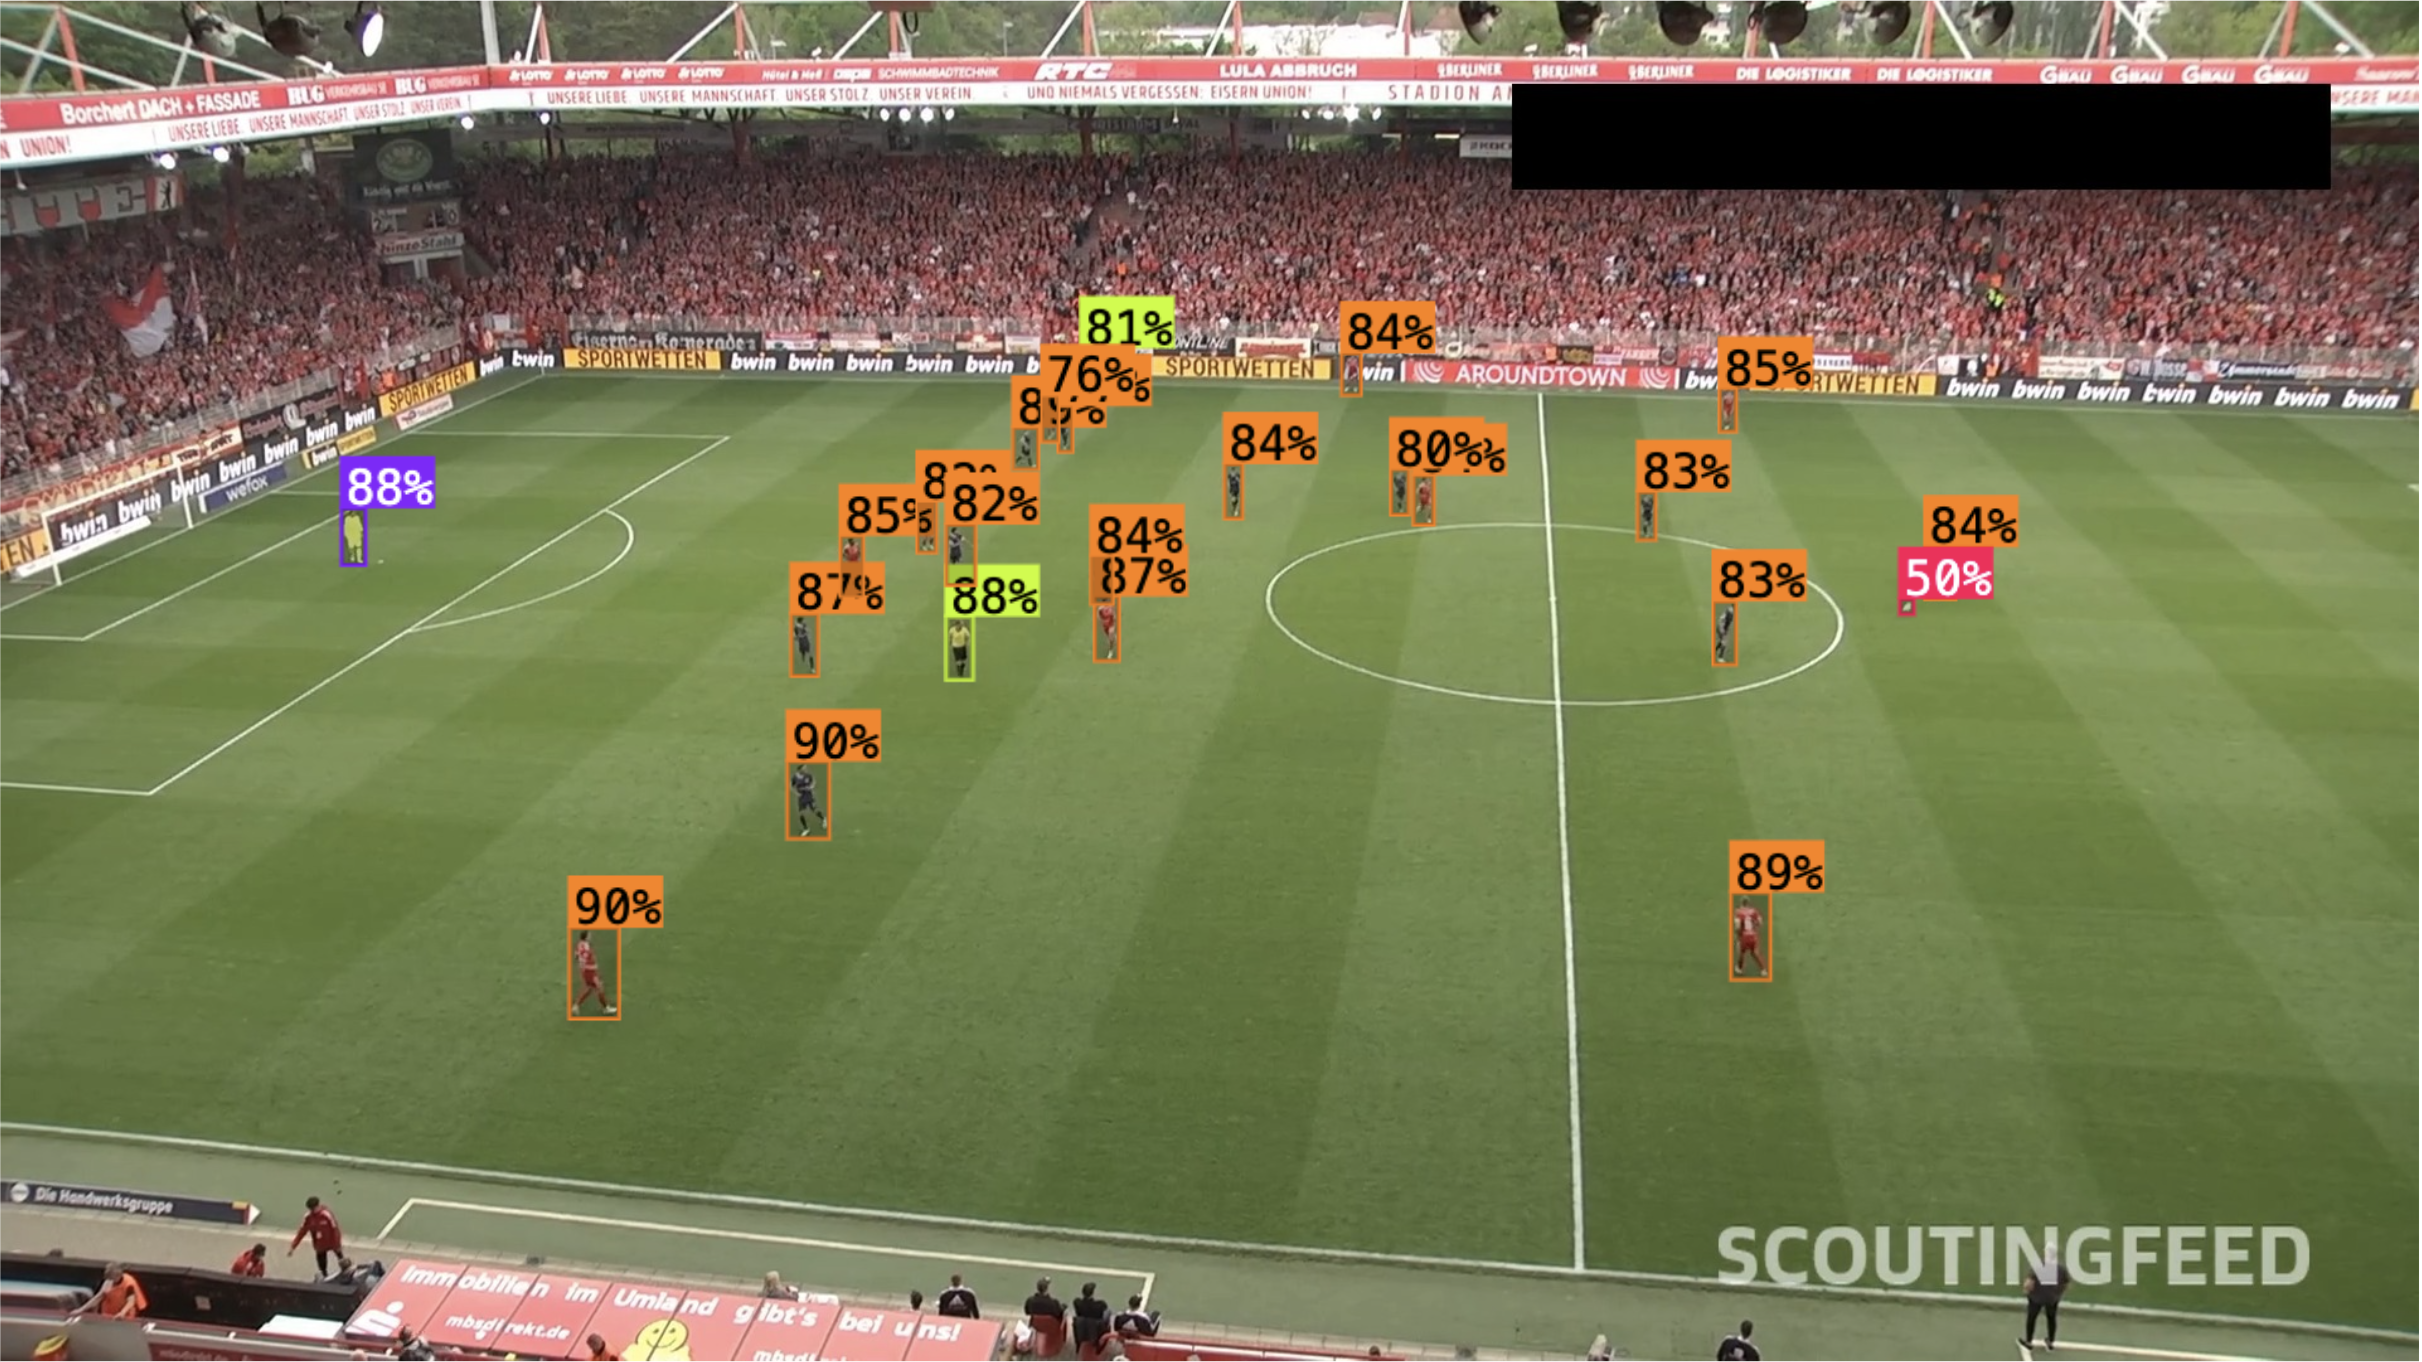
\includegraphics[width=0.7\textwidth]{images/playerDetectionSample.png}
    \caption{Sample Object Detection.}
    \label{fig:playerDetection}
\end{figure}

\subsection{Pitch Keypoint Detection}
\label{subsec:pitchDetectionDesign}

A dedicated \textit{YOLOv8-X} Key-point Detection Model, trained on the labelled pitch data, was employed for the detection of structural field landmarks~\cite{yolov8_ultralytics}. As shown in Figure~\ref{fig:keyPoints}, these include 32 key-points around the pitch, such as the four corners, centre circle extremities, and penalty box vertices. The model outputs 2D coordinates with associated confidence scores for each identified feature.

The training of the model required the selection of hyper-parameters which are talked about as follows:
\begin{enumerate}
    \item \textbf{Epochs:} As stated in Section~\ref{subsec:objectDetectionDesign}, epochs are a key factor in the final model's output. For the pitch detection model, a epoch number of 50 was chosen.
    \item \textbf{Batch Size:} As mentioned previously in Section~\ref{subsec:objectDetectionDesign}, the correct batch size has to be used to strike a balance between speed and stability. Therefore, a batch size of \textbf{16} was opted.
\end{enumerate}


After inference, a confidence threshold is applied to filter out all the low-certainty predictions. This ensures that only the geometrically meaningful and visually reliable key-points are retained. The resulting coordinates are stored as \texttt{supervision.KeyPoints} objects. These objects are used to establish a mapping between a \textit{Bird's Eye View Representation} and their corresponding real-world locations on the pitch which will be talked about later in the report.

\begin{figure}[H]
    \centering
    \includegraphics[width=0.7\textwidth]{images/pitchDetectionSample.png}
    \caption{Sample Pitch Key-Points Detection.}
    \label{fig:pitchDetection}
\end{figure}

Figure~\ref{fig:pitchDetection} shows a sample of the detection of the key-points using the \textit{YOLOv8} Model.

% When a minimum of four high-confidence key-points are available, a homography matrix is computed to project the player and ball positions from the camera frame to a standardized top-down pitch representation, i.e. Bird's Eye View. This transformation is critical for spatial analytics and will be talked about in greater detail in later sections.



\subsection{Player Tracking}
The tracking of players plays a essential role in the overall system, and several other parts depend on it; therefore, tracking should be robust and generate reliable results. The system utilizes \textit{ByteTrack} to achieve this. 

\subsubsection{Why ByteTrack?}
The reason why \textit{ByteTrack} was chosen over other trackers such as \textit{DeepSORT}, is its ability to retain tracking across even the low-confidence detections without requiring appearance embeddings. This makes it more efficient and robust under occlusions. This can be seen in Figure~\ref{fig:ByteTrack}, which showcases \textit{ByteTrack's} performance in comparison to other trackers. In addition, an in detail comparison done by Zhang et al. between \textit{DeepSORT} and \textit{ByteTrack} can be seen in Table~\ref{tab:byte_deepsort_comparison} \cite{zhang2022bytetrack}. Both the models were run using light detection models (\textit{YOLOX}) on the \href{https://motchallenge.net/data/MOT17/}{MOT17 Dataset}.


\begin{figure}[H]
    \centering
    \includegraphics[width=0.7\linewidth]{images/byteTrack.png}
    \caption{Comparison of ByteTrack with other Trackers~\cite{zhang2022bytetrack}.}
    \label{fig:ByteTrack}
\end{figure}



% \begin{table}[H]
% \centering
% \caption{Comparison of BYTE and DeepSORT using light detection models on the MOT17 validation set.}
% \begin{tabular}{@{}lccclcc@{}}
% \toprule
% \textbf{Backbone} & \textbf{Params} & \textbf{GFLOPs} & \textbf{Tracker} & \textbf{MOTA}↑ & \textbf{IDF1}↑ & \textbf{IDs}↓ \\
% \midrule
% YOLOX-M       & 25.3 M & 118.7 & DeepSORT & 74.5 & 76.2 & 197 \\
% YOLOX-M       & 25.3 M & 118.7 & BYTE     & 75.3 & 77.5 & 200 \\
% YOLOX-S       & 8.9 M  & 43.0  & DeepSORT & 69.6 & 71.5 & 205 \\
% YOLOX-S       & 8.9 M  & 43.0  & BYTE     & 71.1 & 73.6 & 224 \\
% YOLOX-Tiny    & 5.0 M  & 24.5  & DeepSORT & 68.6 & 72.0 & 224 \\
% YOLOX-Tiny    & 5.0 M  & 24.5  & BYTE     & 70.5 & 72.1 & 222 \\
% YOLOX-Nano    & 0.9 M  & 4.0   & DeepSORT & 61.4 & 66.8 & 212 \\
% YOLOX-Nano    & 0.9 M  & 4.0   & BYTE     & 64.4 & 68.4 & 161 \\
% \bottomrule
% \end{tabular}
% \label{tab:byte_deepsort_comparison}
% \end{table}


\begin{table}[H]
\centering
\begin{tabular}{|l|c|c|c|c|c|c|}
\hline
\textbf{Backbone} & \textbf{Params} & \textbf{GFLOPs} & \textbf{Tracker} & \textbf{MOTA}↑ & \textbf{IDF1}↑ & \textbf{IDs}↓ \\
\hline
YOLOX-M       & 25.3 M & 118.7 & DeepSORT & 74.5 & 76.2 & 197 \\
YOLOX-M       & 25.3 M & 118.7 & BYTE     & 75.3 & 77.5 & 200 \\
YOLOX-S       & 8.9 M  & 43.0  & DeepSORT & 69.6 & 71.5 & 205 \\
YOLOX-S       & 8.9 M  & 43.0  & BYTE     & 71.1 & 73.6 & 224 \\
YOLOX-Tiny    & 5.0 M  & 24.5  & DeepSORT & 68.6 & 72.0 & 224 \\
YOLOX-Tiny    & 5.0 M  & 24.5  & BYTE     & 70.5 & 72.1 & 222 \\
YOLOX-Nano    & 0.9 M  & 4.0   & DeepSORT & 61.4 & 66.8 & 212 \\
YOLOX-Nano    & 0.9 M  & 4.0   & BYTE     & 64.4 & 68.4 & 161 \\
\hline
\end{tabular}
\caption{Comparison of BYTE and DeepSORT using light detection models on the MOT17 Dataset~\cite{zhang2022bytetrack}.}
\label{tab:byte_deepsort_comparison}
\end{table}


\subsubsection{Implementation}

As mentioned in Section~\ref{subsec:tracking}, ByteTrack is a multi-object tracking algorithm designed to associate detections with persistent object identities across video frames. The tracking was implemented using the aid of the \texttt{supervision} package~\cite{supervision}. The package provided implements a class-based version of the ByteTrack algorithm; using \textit{Kalman Filters} for prediction and the \textit{Hungarian Algorithm} for data association.

% \subsubsection*{Class: \texttt{ByteTrack}}

% \paragraph{Constructor: \texttt{\_\_init\_\_()}}
The ByteTrack tracker has the following configurable parameters:
\begin{itemize}[itemsep=0pt]
  \item \texttt{track\_activation\_threshold}: Minimum confidence score to activate a new track.
  \item \texttt{lost\_track\_buffer}: Maximum number of frames a track can be unmatched before it is removed.
  \item \texttt{minimum\_matching\_threshold}: IoU threshold for data association.
  \item \texttt{frame\_rate}: Video frame rate, used to scale timing behaviour.
  \item \texttt{minimum\_consecutive\_frames}: Required number of frames before considering a track valid.
\end{itemize}

It initializes the Kalman filters and lists to manage the active, lost, and removed tracks. Following this, two functions are used which implement the core of \textit{ByteTrack}.

\paragrpah{Function: \texttt{update\_with\_detections()}}
This function receives the object detector output and returns the tracked results. It:
\begin{enumerate}
  \item Converts bounding boxes and confidence values into tensors.
  \item Passes the tensors to \texttt{update\_with\_tensors()} to update tracking state.
  \item Uses IoU to associate detections with tracked objects and assign them unique tracker IDs.
  \item Returns only detections that were successfully matched to tracks.
\end{enumerate}

\paragraph{Function: \texttt{update\_with\_tensors()}}
This function performs the core tracking logic. It:
\begin{enumerate}
  \item Splits high and low confidence detections into two groups.
  % \item Initializes new \texttt{STrack} objects from high-confidence detections.
  \item Predicts positions of existing tracks using \textit{Kalman Filters}.
  \item Performs data association using \textit{IoU} and the \textit{Hungarian algorithm}.
  \item Matches detections to existing tracks:
  \begin{itemize}
    \item Updates existing tracks.
    \item Re-activates previously lost tracks.
    \item Handles unmatched tracks and detections using a second matching stage with lower confidence detections.
  \end{itemize}
  \item Initializes new tracks from unmatched detections if confidence is high enough.
  \item Prunes tracks that are lost for too long.
\end{enumerate}

% \paragraph{Supporting Functions}
% \begin{itemize}
%   \item \texttt{reset()}: Resets internal tracker state for reuse on new videos.
%   \item \texttt{joint\_tracks()}, \texttt{sub\_tracks()}, \texttt{remove\_duplicate\_tracks()}: Utility functions to manage track lists without duplication.
% \end{itemize}


The ByteTrack implementation in Python efficiently handles multi-object tracking by combining confidence-based filtering, motion prediction, and spatial matching. It offers robustness against detection noise and occlusions and is suitable for real-time sports analytics and video understanding tasks.




\subsection{Team Classification}

\begin{figure}[H]
    \centering
    \includegraphics[width=\linewidth]{images/cropbox.png}
    \caption{Players without Team Classification.}
    \label{fig:cropboxes}
\end{figure}
The classification of players into their respective teams is a highly researched and growing topic in sports analytics. It acts as a crucial pillar for tracking systems and through which insights are given. This system implements team segmentation with the help of the pre-trained \textit{SigLIP} model, \textit{UMAP} Model and K-Means Clustering. The pipeline is explained in detail as follows:
\begin{enumerate}
    \item \textbf{Detecting:} The video frame is given as input and the \textit{YOLOv8} model provides player detections. These detections are vectors which contain the coordinates, width, and height of the box. For the \textit{SigLIP} Model, the input given must be images, therefore the detections are converted to \textit{crop-boxes} which are cropped images of each detection. This can be seen in Figure~\ref{fig:cropboxes}
    \item \textbf{Generating Embeddings:} The crop-boxes are passed through the \textit{SigLIP} model to generate embeddings. These embeddings capture the main semantic meaning of each crop-box, therefore, making the team classification of a player invariant to changes in lighting, position or occlusion.
    \item \textbf{Reducing: } The generated embeddings are of large dimensions, $1 by 768$, and cannot be classified into clusters directly. Therefore, they are passed through the \textit{UMAP Model}, which converts it to \textbf{3-dimensional} vectors, without the loss of information.
    \item \textbf{Clustering: }The 3-dimensional vectors generated from the previous step are clustered into teams with the use of the \textit{K-Means Clustering} algorithm.
\end{enumerate}

This \textit{unsupervised} approach allows team classification without requiring the prior knowledge of the kit colours. 

\subsubsection{Goalkeeper Team Allocation}
Classification of the players can be done based on visual features as they wear the same kit, however, goalkeepers generally wear different coloured kits. As a solution, they are assigned team IDs by calculating distances of the team centroids based on the spatial positioning. The team centroid they are closer to is the one that is assigned to them. This is built on the fact that in football, the teams are as a overall closer to the goalpost they are defending \cite{shaw2019dynamic}.

\begin{figure}[H]
    \centering
    \includegraphics[width=\linewidth]{images/team1.png}
    \includegraphics[width=\linewidth]{images/team2.png}
    \caption{The generated teams after going through the Pipeline.}
    \label{fig:teams}
\end{figure}


\subsubsection{History}
To prevent a player's team being changed frequently, the history of the previously classified team is recorded. Then, the team to which that particular player has been classified to the most is chosen. This prevents the team classification from being susceptible to temporary fluctuations caused by noise in the extraction, occlusions, or lighting inconsistencies. By incorporating this history-based mechanism, the system ensures greater temporal consistency and robustness in team identification, particularly during complex scenes or player interactions where visual features may be unreliable.

\subsection{Pitch Homography and Spatial Mapping}


The \textit{Top-Down View}, also known as \textit{Bird's Eye View}, is crucial in the field of football analytics. It provides a concise and comprehensive spatial awareness of every player on the pitch simultaneously. Unlike broadcast footage focused on either the ball or individual confrontations, an overhead view enables analysts to evaluate team formations, spacing, player positioning, and tactical movements in real-time. This view is necessary for the proper evaluation of strategies like pressing formations, defensive lines, and attacking patterns, in addition to quantifying measurements such as team compactness, pitch control, and passing options. Ultimately, the \textit{Top-Down View} converts the raw video footage into actionable insights, rendering it indispensable for high-level performance analysis and coaching decisions.

As mentioned earlier, a \textit{Key-point Detection Model} detects the pitch key-points. Using the coordinates obtained, a homography matrix is computed using the custom \texttt{ViewTransformer} class to convert between the frame and pitch coordinates. For computation of a homography matrix, a minimum of \textbf{4 points} need to have been detected as explained in Section~\ref{subsec:homography}. Using the \textit{homography matrix}, the key-points are mapped to a known field template obtained from the \texttt{supervision} package (\texttt{SoccerPitchConfiguration}).

This template can be seen in Figure~\ref{fig:2DPitch}. 

\begin{figure}[H]
    \centering
    \includegraphics[width=0.7\linewidth]{images/2DPitch.png}
    \caption{Pitch Template}
    \label{fig:2DPitch}
\end{figure}

This transformation plays a crucial role, enabling:
\begin{itemize}
    \item Top-down projections of the player and ball positions.
    \item Overlaying analytical graphics like offside lines and Voronoi diagrams on the pitch.
    \item Generation of metrics such as player instantaneous speed, cumulative distance, ball possession, and number of passes.
\end{itemize}


\subsection{Generated Heatmaps}

Voronoi diagrams are often used to visualize the spatial control across the pitch. The system can generate two different variations to enhance the overall tactical understanding. Both methods partition the pitch based on the player locations, however, they differ in how the players' presence is visually represented.

\subsubsection{Voronoi Heatmap without Player Markers}

As shown in Figure~\ref{fig:voronoi_no_points}, the first variation displays only the \textit{Voronoi regions} without marking individual players. Each region is colour-coded according to the team's identity, providing a clear visualization of the overall spatial dominance at any given moment without the distraction of specific player positions.

\begin{figure}[H]
    \centering
    \includegraphics[width=0.8\textwidth]{images/heatmap.jpeg}
    \caption{Voronoi Heatmap showing areas of team control without explicit player markers.}
    \label{fig:voronoi_no_points}
\end{figure}

\subsubsection{Voronoi Heatmap with Player Markers}

The second variation can be seen in Figure~\ref{fig:voronoi_with_points}. It overlays player markers onto the Voronoi diagram. Here, each player's position is marked with a distinct dot, offering a more detailed view that connects spatial regions directly to individual players. This version provides a finer insight into the player spacing, clustering, and positioning relative to the controlled regions.

\begin{figure}[H]
    \centering
    \includegraphics[width=0.8\textwidth]{images/heatmap2.jpeg}
    \caption{Voronoi heatmap showing team control areas with individual player markers.}
    \label{fig:voronoi_with_points}
\end{figure}

Both the types of heatmaps are important for analysing the overall team shape and spatial occupation. This allows for both high-level and detailed assessments of the tactical behaviour.





\subsection{Offside Detection}
The rule of offside plays an essential role in the sport of football. The system provides the ability to detect the \textit{offside-line} for both teams and detect if any players stand in the offside position. Before diving into how the \textit{offside-line} is detected, it is crucial to understand what exactly is an offside. Law 11 laid by the \textit{International Football Association Board}, talks about what is classified as an offside. It is stated as follows \cite{ifab2024laws}:\\
\textbf{11.1 Offside Position:} 
\begin{quote}
A player is in an offside position if:
\begin{itemize}
  \item any part of the head, body, or feet is nearer to the opponents' goal line than both the ball and the second-last opponent.
  \item they are in the opponents' half of the field.
\end{itemize}
\textit{Note:} The hands and arms of all players, including the goalkeepers, are not considered. For the purposes of determining offside, the upper boundary of the arm is in line with the bottom of the armpit.
\end{quote}
\textbf{11.2 Offside Offence:} 
\begin{quote}
    A player in an offside position at the moment the ball is played or touched by a team-mate is only penalised on becoming involved in active play by:
\begin{itemize}
  \item interfering with play by playing or touching a ball passed or touched by a team-mate; or
  \item interfering with an opponent by:
    \begin{itemize}
      \item preventing an opponent from playing or being able to play the ball by clearly obstructing the opponent’s line of vision; or
      \item challenging an opponent for the ball; or
      \item clearly attempting to play a ball which is close when this action impacts on an opponent; or
      \item making an obvious action which clearly impacts on the ability of an opponent to play the ball.
    \end{itemize}
  \item gaining an advantage by playing the ball or interfering with an opponent when it has:
    \begin{itemize}
      \item rebounded or been deflected off the goalpost, crossbar, match official or an opponent; or
      \item been deliberately saved by any opponent.
    \end{itemize}
\end{itemize}
\end{quote}
\textbf{11.3 No Offence:} 
\begin{quote}
There is no offside offence if a player receives the ball directly from:
\begin{itemize}
  \item a goal kick;
  \item a throw-in; or
  \item a corner kick.
\end{itemize}
\end{quote}

\textbf{11.4 Sanctions:} 
\begin{quote}
If an offside offence occurs, the referee awards an indirect free kick where the offence occurred, including if it is in the player’s own half of the field of play.
\end{quote}
Based on this law, a basic offside detection algorithm was implemented using concepts of homography to determine the line of offside. 
\begin{enumerate}
    \item Using the concept of homography a \textit{2D Top-Down View}, i.e. Bird's Eye View , is generated.
    \item Based on the team, the player closest to that team's respective goalpost is detected. Note, in this the goalkeeper is excluded as the goalkeeper's position is not taken into account for offside.
    \item A line parallel to the \textit{Y-axis} which passes through the \textit{X}-coordinate of that player is taken. This is the offside line in the Top-down View. This can be seen in Figure~\ref{fig:offside}(a).
    \item The detected offside line is converted to the equivalent line on the live camera pitch using homography. This can be seen in Figure~\ref{fig:offside}(b). 
    \item Any player from the opposition team behind this line without the football in possession is said to be in an \textit{offside position} and is recorded.
    \item If the ball does come in the possession of a player in an \textit{offside position} it is classified as an \textit{offside offence}. In response, a free kick is given to the defending team.
\end{enumerate}

\begin{figure}[H]
    \centering
    \begin{subfigure}[b]{\linewidth}
        \centering
        \includegraphics[width=\linewidth]{images/offside2D.jpeg}
        \caption{Offside line detection on 2D pitch view.}
        \label{fig:offside-2d}
    \end{subfigure}
    \hfill
    \\
    \begin{subfigure}[b]{\linewidth}
        \centering
        \includegraphics[width=\linewidth]{images/offside.png}
        \caption{Offside line detection on broadcast view.}
        \label{fig:offside-broadcast}
    \end{subfigure}
    \caption{Sample images with the offside line detected in different views.}
    \label{fig:offside}
\end{figure}


As seen in Figure~\ref{fig:offside}, the offside line was detected from the 2D view and then using homography, the line was converted to fit on the live camera pitch. The reason why the detection of the offside line is done on the \textit{Top-Down View} and not directly on the live camera is that the offside line has to be parallel to the pitch, however, the pitch is seen from a particular angle. Therefore, detection of it is much simpler if done on the \textit{Top-Down View},
\subsection{Tactical Analysis}

The system adds another feature of tactical analysis. Tactical analysis provides great aid in understanding the game. It gives insights into the players individual performances and can identify key takeaways, one that might go unnoticed by the human eye. A thorough analysis of each frame is done and through this the multiple metrics are obtained.

\subsubsection{Possession}
The possession of the ball is determined by the proximity of the player to the ball. The player closest to the ball is said to be in possession of the ball, however, a maximum threshold value for the distance is applied. If distance between the ball and the closest player is larger than this, the player is not considered to be in possession of the ball. A threshold value was implemented as the ball can be in the air or even passed, and during the travel, the ball is said to be in no one's possession. 

The apt value for the threshold value was determined to be \textbf{40px}, as it was calculated to be an equivalent of around 3 meters. In real life, if the ball was more than 3 meters away from the player, they would not be said to be in possession. This is very basic methodology, and they can be multiple instances where the player might be sprinting and the ball might exceed the threshold but still be in possession, however, this was generally found to be apt.

This concept aided in two additional statistics; \textit{Team Possession Percentage} and \textit{Number of Passes}.

Whenever a player was considered to be in the possession of the ball, it was recorded. Finally, after each and every frame has been examined, the overall possession percentage of each team was calculated using the following formula:
\[
P_{\text{team}} = \frac{F_{\text{team}}}{F_{\text{total}}} \times 100
\]
where:
\begin{itemize}
    \item $F_{\text{team}}$ is the total number of frames where a player from the team was recorded in possession,
    \item $F_{\text{total}}$ is the total number of frames where any player was recorded in possession.
\end{itemize}

In a similar manner the \textit{number of passes by a team} was also estimated. If the possession of the ball changes, and the new player in possession is of the same team, it was considered as a \textbf{pass}. The number of passes completed by each team was recorded and displayed at the end. It is important to note here that this was a very simple method and does not take into consideration tackles and non-intentional passes.

\subsubsection{Player Speed and Distance Coverage}
To analyse the player performance, the speed and total distance covered by each player over the course of the match was calculated. This gave a great insight into the individual performance of players, a very helpful analysis for coaches. The instantaneous speed and total distance travelled was obtained by tracking the player's movements across frames in the 2D broadcast view. Each player's positional changes were computed using their coordinates extracted from the homography-transformed \textit{Top-Down View} of the pitch.
camera perspectives and zoom levels in broadcast footage we normalized these positional changes 
Given the variation in pitch sizes based on the location, an assumption was made. It was assumed that the pitch was an average real-world pitch dimension of $105 \times 68$ meters, in line with FIFA regulations for a standard football field. The scaling factor between image pixels and real-world meters was estimated based on the pitch corners identified through key-point detection and homography estimation.

The distance $d$ travelled between two consecutive frames was calculated using the Euclidean distance formula:
\[
d = \sqrt{(x_2 - x_1)^2 + (y_2 - y_1)^2}
\]
where $(x_1, y_1)$ and $(x_2, y_2)$ are the coordinates of the player in successive frames, mapped to real-world coordinates.

Cumulative distance for each player was then obtained by summing these per-frame distances across the entire match. The instantaneous speed $v$ of a player was estimated by:
\[
v = \frac{d}{\Delta t}
\]
where $\Delta t$ is the time interval between frames, determined using the video's frame rate (e.g., $\Delta t = \frac{1}{25}$ seconds for a 25 fps video).

This methodology provides an overall reliable approximation of the player dynamics; enabling insights into the player workload, sprinting bursts, and positioning during different phases of the game.



% \subsubsection{Video Processing Pipeline}

% The system processes video frames in the following pipeline:

% \begin{enumerate}
%     \item Generate frames from video source using a stride.
%     \item Apply object detection and tracking.
%     \item Run team classification and pitch homography.
%     \item Annotate each frame with tactical overlays.
%     \item Write results to disk using \texttt{cv2.VideoWriter} or \texttt{supervision.VideoSink}.
% \end{enumerate}

% Different output streams are supported: raw detection overlays, top-down tactical views, Voronoi maps, offside visuals, and statistical overlays.

% \bigskip

% This modular and scalable pipeline ensures real-time feasibility, robustness to partial occlusion, and flexibility for integration into future tactical applications.


\newpage


%%%%%%%%%%%%%%%%%% RESULTS %%%%%%%%%%%%%%%%%%
\section{Evaluation and Results} \label{sec:results}



This chapter present a detailed evaluation of each component of the system; player detection, pitch detection, team classification, and tracking performance. Several hyper-parameters have been experimented with to obtain the optimum fine-tuned model for each component. Metrics such as \textbf{mean Average Precision (mAP)} and \textbf{Higher Order Tracking Accuracy (HOTA)} have been used to quantify performance.

\subsection{Common Metrics}
For the evaluation of different components, several different metrics were used. Some of the common ones are explained here briefly:
\begin{enumerate}
    \item \textbf{Accuracy} measures the proportion of correctly predicted instances (both true positives and true negatives) among all instances.
\begin{equation}
\text{Accuracy} = \frac{TP + TN}{TP + TN + FP + FN}
\end{equation}

\item \textbf{Precision} measures the proportion of true positive predictions among all positive predictions.
\begin{equation}
\text{Precision} = \frac{TP}{TP + FP}
\end{equation}

\item \textbf{Recall} (also known as Sensitivity or True Positive Rate) measures the proportion of true positives among all actual positives.
\begin{equation}
\text{Recall} = \frac{TP}{TP + FN}
\end{equation}

\item \textbf{F1 Score} is the harmonic mean of Precision and Recall, providing a balance between the two.
\begin{equation}
\text{F1 Score} = 2 \times \frac{\text{Precision} \times \text{Recall}}{\text{Precision} + \text{Recall}}
\end{equation}

\noindent
Where:
\begin{itemize}
    \item \( TP \) = True Positives
    \item \( TN \) = True Negatives
    \item \( FP \) = False Positives
    \item \( FN \) = False Negatives
\end{itemize}
\end{enumerate}

\item \textbf{Mean Average Precision (mAP@0.5):} This measures the trade-off between precision and recall at an Intersection over Union (IoU) threshold of 0.5. A higher mAP indicates better detection performance.

\subsection{Object and Key-Point Detection}

\subsubsection{Data Preparation}

Proper data preparation is essential to ensure an overall fair evaluation of the components. The dataset collected for this project's evaluation consists of annotated football frames containing bounding boxes for the players, referees, the ball, and pitch key-points. The following data splits were used:

\begin{itemize}
    \item \textbf{Training Set:} 80\% of the total labelled frames
    \item \textbf{Validation Set:} 10\% of the total labelled frames
    \item \textbf{Test Set:} 10\% of the total labelled frames
\end{itemize}

Frames were randomly shuffled before splitting to avoid temporal correlation between frames from the same sequence. Data augmentation strategies such as random horizontal flipping, noise, blur, contrast and brightness changes, and mosaic composition were applied during training but not during validation or testing. This ensures that model evaluation accurately reflects performance on real-world, unseen data without augmentation artifacts. This ensures that the result obtained are reliable and depict an honest evaluation.

\subsubsection{Evaluation Metrics}
The primary metrics used for evaluating the detection models are \textbf{accuracy}, \textbf{precision}, and \textbf{mAP@0.5}.

\subsubsection{Player Detection}
Accurate player detection is critical as it underpins all downstream components such as tracking, team classification, and tactical analysis. Any inaccuracies in the detections would directly affect the performance of subsequent modules.

\paragraph{Experimentation and Results}
The detection of players, referees, and the ball is the primary steps and requires a robust object detection model. To obtain a reliable \textit{YOLO} model, experimentation with various different configurations was performed:

\begin{enumerate}
    \item \textbf{Low Resolution + No Augmentation:} A lower resolution of \[640 \times 640\] was used. No data-augmentation was done here.
    \item \textbf{High Resolution + No Augmentation}: A higher resolution of \[1280 \times 1280\] was used. No data-augmentation was done here.
    \item \textbf{Default Augmentation:} The default augmentation of data done by \textit{YOLOv8} was used here. This includes: 
    \begin{itemize}
      \item \textbf{Hue }: Random Hue shift up to $\pm0.015$.
      \item \textbf{Saturation}: Saturation scaled by a factor up to 0.7.
      \item \textbf{Brightness}: Brightness scaled by a factor up to 0.4.
      \item \textbf{Translation}: Random shift in x and y direction up to $\pm10\%$ of image size.
      \item \textbf{Scaling}: Image scaled randomly by a factor up to 0.5.
      \item \textbf{Horizontal Flip}: Applied with 50\% probability.
      \item \textbf{Mosaic Augmentation}: Combines four images into one training sample.
    \end{itemize}
    \item \textbf{Improved Augmentation:} The default augmentation of data done by \textit{YOLOv8} was improved by changing a few values making it for football. This includes: 
    \begin{itemize}
      \item \textbf{Rotation}: Randomly rotated up to $\pm10^\circ$
      \item \textbf{Shear}: Shear was randomly added from $\pm10^\circ$ \textit{horizontal} and $\pm10^\circ$ \textit{vertical}.
      \item \textbf{Brightness}: Brightness was varied by $\pm15\%$.
      \item \textbf{Exposure}: Exposure was varied by $\pm10\%$.
     \item \textbf{Blur}: Blur was added up to by $0.7 px$.
      \item \textbf{Horizontal Flip}: Applied with 50\% probability.
      \item \textbf{Mosaic Augmentation}: Combines four images into one training sample.
    \end{itemize}
    \item \textbf{Mixup+Augmentation:} This has the same augmentation as the previous but also adds mixup. In mixup, the images are overlaid with weighted transparency of other images. This aids in the overall regularization of the model.



\end{enumerate}

\begin{table}[H]
\centering
\begin{tabular}{|l|c|c|c|}
\hline
\textbf{Configuration} & \textbf{mAP@0.5} & \textbf{Recall} & \textbf{Precision} \\
\hline
Low Resolution & 80.8\% & 76.3\% & 87.2\% \\
High Resolution + No Augmentation & 87.8\% & 85.9\% & 88.1\% \\
Default Augmentation & 90.7\% & 84.9\% & 93.4\% \\
Improved Augmentation & 90.9\% & 85.7\% & 93.5\% \\
Augmentation + Mixup & 90.9\% & 86.8\% & 91.4\% \\
\hline
\end{tabular}
\caption{Object Detection Model Results for change in Augmentation.}
\label{tab:player_detection_results}
\end{table}

A secondary experiment was done. The learning rate plays a great role in the overall functioning of the model. It decides by how much should the weights change after each epoch. 
\begin{table}[H]
\centering
\begin{tabular}{|l|c|c|c|}
\hline
\textbf{Learning Rate} & \textbf{mAP@0.5} & \textbf{Recall} & \textbf{Precision} \\
\hline
0.001 & \textbf{91.1\%} & 86.2\% &\textbf{ 95.1\%} \\
0.01 & 90.9\% & 85.7\% & 93.5\% \\
0.1 & 90.1\% & \textbf{88.7\%} & 87.8\% \\
\hline
\end{tabular}
\caption{Object Detection Model Results for change in Learning Rate.}
\label{tab:player_detection_results}
\end{table}

A graph has also been shown displaying the training of the final model with \textbf{augmentation} and a learning rate of \textbf{0.001}.
\begin{figure}[H]
    \centering
    \includegraphics[width=0.6\linewidth]{images/objectdetectiongraph.png}
    \caption{Graphs showing the training of the Object Detection Model. Contains Precision, Recall, mAP@0.5 and mAP@0.5-0.95. The x-axis represnts the epoch number.}
    \label{fig:pitchDetectionResults}
\end{figure}

\subsubsection{Discussion}
The results demonstrate that training on low resolution despite using less resources does not produce accurate enough results. It struggles especially in ball detections where the ball gets blurred too much due to the resizing. In addition, extensive augmentation techniques combined with mix-up, significantly improved the model's ability to generalize to unseen football frames. Therefore, the the model was trained on augmented data with mix-up.

From the secondary experiment it can be seen that a lower learning rate does improve the model generating a significant improvement in \textit{mAP@0.5}. This shows that slowly converging to the minima of loss function obtains better results here, however, at the cost of resources. Higher learning rates do often cause the model to overshoot and diverge from the optimum solution.

\subsubsection{Pitch Detection}
Pitch detection is a fundamental part that enables spatial transformations such as pitch homography, crucial for creating tactical bird's-eye views and spatial analyses.

\subsubsection{Evaluation Metrics}
The pitch detection model was evaluated using \textbf{mAP@0.5}.

\subsubsection{Experimentation and Results}
The pitch detection model was evaluated by varying the number of epochs. Epochs was chosen here as it showcases if the model might be over-fitting or under-fitting; a factor that plays a significant role in key-point localization. The values \textbf{100, 300, }and\textbf{ 500} were tested. The results are displayed below.

\begin{table}[H]
\centering
\begin{tabular}{|l|c|c|c|}
\hline
\textbf{Epoch Number} & \textbf{Precision} & \textbf{Recall} & \textbf{mAP@0.5} \\
\hline
100 &  99.8\% & 100\% & 99.5\%\\
300 & 100\% & 100\% & 99.5\%\\
500 & 99.9\% & 100\% & 99.5\%\\
\hline
\end{tabular}
\caption{Pitch Detection Performance on Different Epochs.}
\label{tab:pitch_detection_epoch}
\end{table}

A graph has also been shown displaying the training of the 300 epochs model.
\begin{figure}[H]
    \centering
    \includegraphics[width=0.6\linewidth]{images/pitchDetectionResults.png}
    \caption{Graphs showing the training of the Pitch Detection Model. Contains Precision, Recall, mAP@0.5 and mAP@0.5-0.95. The x-axis represnts the epoch number.}
    \label{fig:pitchDetectionResults}
\end{figure}

\subsubsection{Discussion}
Unlike object detection, it can be seen here that even lower-resolution images generate highly accurate models, therefore eliminating the need to run on higher quality images at the cost of resources. 

The results show that by applying a combination of different augmentations during training leads to significant improvements in the keypoint localization. The correct number of epochs improves the performance of the model by a \textbf{0.1\%} Precision. Even though the improvement might not seem great, in high-resolution football videos, even minute errors can lead to distort spatial mappings.

\subsection{Team Classification}
Team classification is a crucial component in sports video analytics. It plays a key role in tactical analysis and off-side detection.

\subsubsection{Data Collection}
For the testing of the player classification, testing was done using from the validation data of 
\href{https://motchallenge.net/data/MOT17/}{\textbf{MOT17 Dataset - MOTChallenge}}. The ground truth provided was compared with the result of the classification pipeline


\subsubsection{Evaluation Metrics}
Team classification performance was evaluated using \textbf{accuracy}, \textbf{precision}, \textbf{recall}, and \textbf{F1 Score}.
\subsubsection{Experimentation and Results}
The overall team classification's results can be seen below:
\begin{table}[H]
\centering
\begin{tabular}{|c|c|}
\hline
\textbf{Metric} & \textbf{Value} \\
\hline
Accuracy & 0.9583678541839271 \\
Precision & 0.9638345089677017 \\
Recall & 0.9539961886863946 \\
F1 Score & 0.9575176656228064 \\
\hline
\end{tabular}
\caption{Overall Performance Metrics}
\label{tab:classification results}
\end{table}


\subsubsection{Discussion}
Based on the results obtained, we can conclude that the overall algorithm for team segmentation works efficiently even when the conditions can vary significantly.

\subsection{Player Tracking}
As mentioned previoulsy in Subsection~\ref{subsec:tracking}, player tracking plays a key role and therefore it needs to be reliable. To ensure this, it was evaluated extensively, testing multiple different parameters of it. The variables experimented with are as follows:
\begin{enumerate}
    \item \textbf{Minimum Matching Threshold:} This represents the minimum IoU-based threshold to match detections with existing tracks.
    The following values were tested: \textbf{0.7, 0.8, 0.9}.
    \item \textbf{Track Activation Threshold:} This is the confidence threshold for a detection to start tracking.
    The following values were tested: \textbf{0.1, 0.25, 0.4}.
    \item \textbf{Minimum Consecutive Frames:} This is the minimum number of frames before a track is considered valid.
    The following values were tested: \textbf{1, 2, 3}.
\end{enumerate}

Each parameter was individually experimented with, keeping the other parameters to their default value.


\subsubsection{Data Collection}
Similar to player classification, the evaluation of the player tracking was done on the validation data of 
\href{https://motchallenge.net/data/MOT17/}{\textbf{MOT17 Dataset - MOTChallenge}}. The tests were run using the code given by \href{https://github.com/MCG-NJU/SportsMOT/tree/main}{\textit{SportsMOT}}.


\subsubsection{Evaluation Metrics}
Tracking performance was quantified using \textit{HOTA (Higher Order Tracking Accuracy)}.

While \textit{Multiple Object Tracking Accuracy (MOTA)} has been a longstanding standard for evaluating tracking systems, it presents several critical limitations for modern, complex tracking scenarios. \textit{MOTA} primarily emphasizes detection errors (false positives and false negatives) and identity switches. This results in a metric that heavily weights \textit{detection performance} over \textit{association accuracy}. This imbalance often leads to misleading evaluations where trackers that excel at maintaining consistent identities across frames are unfairly penalized if they have minor detection issues~\cite{hota}.

Furthermore, \textit{MOTA’s} association scoring is limited to short-term, first-order errors and does not capture long-term identity consistency, which is crucial in sports analytics where player tracking must remain accurate across the duration of the match.

To address these deficiencies, \textit{HOTA (Higher Order Tracking Accuracy)}. Unlike \textit{MOTA}, \textit{HOTA} evaluates both detection and association with equal weighting. It achieved this by measuring the association accuracy over entire trajectories rather than just between consecutive frames. This higher-order association analysis allows HOTA to more accurately reflect how well predicted tracks align with the ground truth over time~\cite{hota}.

% It also handles ID switches more intuitively, rewarding trackers that are able to recover from earlier mistakes---something MOTA fails to do, as it penalizes corrections as if they were new errors. Additionally, HOTA’s use of the Jaccard index ensures the metric is symmetric and bounded, offering a clearer and more interpretable evaluation score.

For these reasons, HOTA was selected as a more balanced and insightful evaluation metric for evaluating the tracking performance of the system. However, the metric \textit{MOTA} is also given for comparison purposes.


\textit{HOTA} is defined as the average of the geometric mean of the detection accuracy \textit{(DetA)} and the association accuracy \textit{(AssA)} across a range of \textit{IoU} thresholds:

\begin{equation}
\mathrm{HOTA} = \frac{1}{|\mathcal{A}|} \sum_{\alpha \in \mathcal{A}} \sqrt{\mathrm{DetA}(\alpha) \cdot \mathrm{AssA}(\alpha)}
\end{equation}

Where:
\begin{itemize}
    \item $\mathcal{A}$ is a set of IoU thresholds (e.g., $\{0.05, 0.10, ..., 0.95\}$)
    \item $\alpha$ is the specific IoU threshold
    \item $\mathrm{DetA}(\alpha)$ is the detection accuracy at threshold $\alpha$
    \item $\mathrm{AssA}(\alpha)$ is the association accuracy at threshold $\alpha$
\end{itemize}

These components are defined as follows:
\begin{enumerate}
    \item Detection accuracy measures how well the tracker finds objects (i.e., players) in each frame:

\begin{equation}
\mathrm{DetA}(\alpha) = \frac{|\mathrm{TP}_{\alpha}|}{|\mathrm{TP}_{\alpha}| + |\mathrm{FP}_{\alpha}| + |\mathrm{FN}_{\alpha}|}
\end{equation}

Where:
\begin{itemize}
    \item $\mathrm{TP}_{\alpha}$ = true positives at IoU $\alpha$ (correctly matched detections)
    \item $\mathrm{FP}_{\alpha}$ = false positives at IoU $\alpha$ (extra detections)
    \item $\mathrm{FN}_{\alpha}$ = false negatives at IoU $\alpha$ (missed detections)
\end{itemize}

In simple terms: \textit{DetA tells us how many players were correctly detected compared to how many were missed or wrongly added.}


\item Association accuracy measures how well the tracker maintains the identity of each object over time:

\begin{equation}
\mathrm{AssA}(\alpha) = \frac{1}{|\mathrm{TP}_{\alpha}|} \sum_{c \in \mathrm{TP}_{\alpha}} \mathcal{A}(c)
\end{equation}

Where:
\begin{itemize}
    \item $\mathcal{A}(c)$ is the association score for a correct match $c$, which evaluates how well the tracker's identity for that object matches the ground truth identity across its trajectory.
\end{itemize}

In plain terms: \textit{AssA tells us how good the system is at keeping the same ID for each player across frames—crucial for analyzing movement and strategy.}
\end{enumerate}


\vspace{1em}

By combining detection accuracy and association accuracy at multiple IoU levels, HOTA provides a balanced view of both how \textit{accurate} and how \textit{consistent} a tracker is. It overcomes the limitations of older metrics like MOTA, which focus too much on detection and not enough on identity tracking.




\subsubsection{Experimentation and Results}
Experiments were conducted to tune the ByteTrack tracker settings. Various parameters were tested as mentioned and an overall combination was chosen. 

\begin{table}[H]
\centering
\begin{tabular}{|c|c|c|}
\hline
\textbf{Minimum Matching Threshold} & \textbf{MOTA (\%)} & \textbf{HOTA (\%)} \\
\hline
0.7 & 81.397\% & 66.544\%\\
0.8  &  82.961\% &  71.413\% \\
\textbf{0.9} & \textbf{83.738\%} & 72.953\%\\ 
\hline
\end{tabular}
\caption{Tracking Performance Results for Minimum Matching Threshold.}
\label{tab:matching_threshold}
\end{table}

\begin{table}[H]
\centering
\begin{tabular}{|c|c|c|}
\hline
\textbf{Track Activation Threshold} & \textbf{MOTA (\%)} & \textbf{HOTA (\%)} \\
\hline
0.1 & 82.943\% & 71.407\%\\
0.25 & 82.961\%  &  71.413\% \\
\textbf{0.4} & \textbf{83.092\%} &  \textbf{71.481\%} \\
\hline
\end{tabular}
\caption{Tracking Performance Results for Track Activation Threshold.}
\label{tab:activation_threshold}
\end{table}


\begin{table}[H]
\centering
\begin{tabular}{|c|c|c|}
\hline
\textbf{Minimum Consecutive Frames} & \textbf{MOTA (\%)} & \textbf{HOTA (\%)} \\
\hline
\textbf{1} & \textbf{82.961\%} &  \textbf{71.413\%} \\
2 &  80.14\% & 70.28\%\\
3 & 79.616\% & 69.65\% \\ 
\hline
\end{tabular}
\caption{Tracking Performance Results for Minimum Consecutive Frames.}
\label{tab:consecutive_frames}
\end{table}



\subsubsection{Discussion}
From the results, it can be clearly seen that adjustments to parameters significantly affected the results. From the experiment, we can see that an overall high threshold 
value for matching to be considered valid generates better results. Similarly, a higher threshold value for the activation of a track creates more reliable outputs. However, in contrast to the previous two, a lower number for the minimum frame required for a track to be considered valid has generated the best results. 
 
The parameters were then combined with their best values: 
 \begin{enumerate}
     \item Minimum Matching Threshold: \textbf{0.9}.
     \item Track Activation Threshold: \textbf{0.4}
     \item Minimum Consecutive Frames: \textbf{1}.
 \end{enumerate}
 
The final system obtained produced a \textit{HOTA} of \textbf{73.044\%} and a \textit{MOTA} of \textbf{83.921\%}. 

\subsection{General Discussion}
From the evaluation results across all components, we can demonstrate that:

\begin{itemize}
    \item Strong data augmentation is essential for improving the robustness of \textit{object} and \textit{keypoint detection} models.
    \item Tracking can be significantly improved by using models to generate embeddings over traditional methods.
    \item Fine-tuning tracker parameters significantly improves tracking stability, especially in complex football scenes involving occlusions and rapid player movements.
\end{itemize}

Future work could involve deploying larger detection backbones, exploring semi-supervised clustering for team classification, and incorporating temporal smoothing modules into the tracking pipeline to further enhance system reliability.

\newpage

%%%%%%%%%%%%%%%%%% CONCLUSIONS %%%%%%%%%%%%%%%%%%
\section{Conclusions and Reflections}
This chapter concludes the overall project by discussing the key achievements, difficulties experienced, personal reflections and learnings and future work in the field. It provides an overview of the full project and hopes to pave a path for projects in the future to ensure the field continues to grow.

\subsection{Summary of Achievements}
The key achievements of this football video analysis system include:
\begin{itemize}
    \item \textbf{Object Detection and Tracking:} A \textit{YOLO}-based object detection pipeline tailored to football environments was successfully deployed. This was combined with a \textit{ByteTrack} tracking system for real-time, identity-consistent player tracking.
    \item \textbf{Team Classification:} The development of a robust team classification method using \textit{SigLIP vision embeddings, UMAP dimensionality reduction, }and \textit{K-Means clustering} was achieved.
    \item \textbf{Pitch Homography:} Accurate mapping of player positions from the broadcast view to a standardised top-down pitch representation using automatic keypoint detection and a robust homography estimation was made possible.
    \item \textbf{Advanced Annotations:} Novel features such as offside detection through automated identification of last defenders, possession tracking based on ball proximity, and player instantaneous speed and cumulative distance were successfully implemented. This enhanced the system's ability to generate tactical insights that could aid in multiple ways.
    \item \textbf{Spatial Analytics:} Voronoi heatmaps and positional density plots to visualise team dominance and player occupation zones across the pitch were generated.
    % \item \textbf{System Design:} Building the project using object-oriented programming principles, ensuring extensibility, maintainability, and clarity of the codebase.
\end{itemize}

Collectively, these achievements have culminated in a highly effective and comprehensive system that addresses a wide spectrum of analytical needs for football video analysis.

\subsection{Notable Challenges}

Several significant challenges were encountered during the development lifecycle. They are mentioned as follows:
\begin{itemize}
    \item \textbf{Data Collection and Annotation:} The lack of readily available labelled tactical camera footage raised an issue. It led to an intensive manual effort required for accurate frame-by-frame annotation of players, balls, referees, and pitch key-points posed an early bottleneck.
    \item \textbf{Robustness of Detection:} Handling occlusions, overlaps, and varied lighting conditions during object detection was a persistent challenge. Solutions included data augmentation and hyper-parameter tuning to improve the overall model.
    \item \textbf{Team Classification Complexity:} Developing a clustering pipeline capable of reliably separating teams required the use of advanced feature embeddings and dimensionality reduction techniques beyond traditional colour histograms.

    % \item \textbf{Performance Optimisation:} Balancing model accuracy with inference speed was critical for maintaining real-time processing capabilities, especially when integrating multiple deep learning models concurrently.
    \item \textbf{Resource Limitation:} Testing multiple different hyper-parameters to obtain the best model performance required extensive resources. Often training of models went up to 5 hours even with the use of \textit{GPU(Graphics Processing Unit)}. With a limited number of free hours on cloud-based \textit{Jupyter notebook} environments, this was often a challenge faced.
\end{itemize}

These challenges necessitated iterative problem-solving, with several architectural redesigns and multiple experimentation cycles required to refine the final system.

\subsection{Self-Reflection}
The project provided a great experience teaching a number of different things. The key reflections are noted as follows:
\begin{enumerate}
    \item \textbf{Planning:} Upon reflection after the completion of the project, a key part to achieving the system was a careful and in-detail planing. Without the understanding and planning of the overall components and estimation of the time it would take for completion, the final system of such stature would have been achieved. Balancing out the independent research required, the overall organization, and the implementation was needed to be done to obtain the best results.
    \item{Pipeline Implementation:} Throughout the project, a profound understanding of the interplay between theoretical knowledge and practical implementation was developed. Early assumptions about the simplicity of integrating separate modules into a unified pipeline were quickly challenged. This highlighted the complexities associated with the consistency of data flow, asynchronous video frame handling, and modular interdependence.
    \item{Model Training:} The iterative nature of deep learning model development was learnt. Performance gains were often incremental and required minute adjustments rather than large changes. The practical realities of computer vision deployment led to a deeper appreciation of robust evaluation strategies and error analysis.
\end{enumerate}



\subsection{Future Work}
The analysis of sports is an evergreen field and shall continue growing. This project has only tapped into the field and there is much more to be achieved. A few of the avenues for future enhancement of the system have been mentioned below:
\begin{itemize}
    \item \textbf{Larger Datasets:} Larger Datasets could significantly improve the overall model. High-quality data showcasing different situations in the game could make the model more robust and provide better results.
    \item \textbf{Deep Re-Identification Models:} Incorporating dedicated player re-identification models could further reduce tracking identity switches during player occlusions and collisions.
    % \item \textbf{Transformer-Based Detection:} Exploring transformer-based object detection models (such as DINO or YOLOv9) may yield improvements in small object detection accuracy and better generalisation across broadcast variations.
    \item \textbf{Pose Estimation Integration:} Integrating human pose estimation alongside bounding boxes could provide finer-grained understanding of the player movements and stances, enriching tactical analysis. It could also improve the overall detections of offside.
    \item \textbf{Multi-View Fusion:} Expanding the system to handle multi-camera input and perform view fusion could unlock richer 3D reconstructions and more accurate player localisation as well as tracking.
    \item \textbf{Action Identification:} Building models that can detect different actions performed by players such as passes, attempted shots, and tackles can provide great insights to coaches and even the common man. In addition, detection of events on the field such as penalties, free-kicks, fouls could improve the game overall.
    \item \textbf{Adaptation to other sports:} There are several other sports for which a similar system can be developed. From cricket to rugby each sport has its own style and specifications which would need to be taken into consideration.

\end{itemize}

By pursuing these directions, the system's capabilities could be expanded beyond the current pipeline into a fully-fledged tactical analysis suite for professional football teams and broadcasters.

\subsection{Conclusion}

In conclusion, this project has successfully demonstrated the feasibility and effectiveness of an integrated football video analytics system, one that is capable of producing detailed tactical insights from raw broadcast footage.

We have been able to implement a system that can detect players, referees and the ball with great accuracy. An efficient and robust tracker has been utilized to obtain reliable results. Classification of the players into their respective teams showcases The system further boasts of the ability to generate spatial analysis by outputting \textit{Voronoi heatmaps}. Finally the system adds a layer of tactical analysis by showcasing ball possession, individual player speed and distance travelled, and offside detection.

By addressing complex challenges in different components, a strong foundation has been established for future development and research in automated sports analytics. The experience gained during this project has provided a an overall hunger for deeper exploration of computer vision, machine learning, and sports data science in real-world applications. 

The project as a whole has achieved its aims and objectives and provides a valuable stepping stone in the field of analytics. As the future work suggests, there is always a potential for improvement; to generate better and more in-depth analysis of the sport, for the coaches and the common crowd. 



%%%%%%%%%%%%%%%%%% REFERENCES %%%%%%%%%%%%%%%%%%
%\clearpage % uncomment to start on a new page if wanted
\printbibliography[title={References},heading=bibintoc] % a single list of references for the whole thesis



%%%%%%%%%%%%%%%%%% APPENDICES %%%%%%%%%%%%%%%%%%
% \begin{uomappendix} 
%     \section{Project outline}
%     Project outline as submitted at the start of the project is a required appendix. Put here. 
    
%     \section{Risk assessment}
%     Risk assessment is a required appendix. Put here.
    
%     %\subsection{Other appendices as necessary}
% \end{uomappendix}


%%%%%%%%%%%%%%%%%% END MATTER %%%%%%%%%%%%%%%%%%
\end{document}
